\documentclass[twoside]{book}

% Packages required by doxygen
\usepackage{fixltx2e}
\usepackage{calc}
\usepackage{doxygen}
\usepackage[export]{adjustbox} % also loads graphicx
\usepackage{graphicx}
\usepackage[utf8]{inputenc}
\usepackage{makeidx}
\usepackage{multicol}
\usepackage{multirow}
\PassOptionsToPackage{warn}{textcomp}
\usepackage{textcomp}
\usepackage[nointegrals]{wasysym}
\usepackage[table]{xcolor}

% Font selection
\usepackage[T1]{fontenc}
\usepackage[scaled=.90]{helvet}
\usepackage{courier}
\usepackage{amssymb}
\usepackage{sectsty}
\renewcommand{\familydefault}{\sfdefault}
\allsectionsfont{%
  \fontseries{bc}\selectfont%
  \color{darkgray}%
}
\renewcommand{\DoxyLabelFont}{%
  \fontseries{bc}\selectfont%
  \color{darkgray}%
}
\newcommand{\+}{\discretionary{\mbox{\scriptsize$\hookleftarrow$}}{}{}}

% Page & text layout
\usepackage{geometry}
\geometry{%
  a4paper,%
  top=2.5cm,%
  bottom=2.5cm,%
  left=2.5cm,%
  right=2.5cm%
}
\tolerance=750
\hfuzz=15pt
\hbadness=750
\setlength{\emergencystretch}{15pt}
\setlength{\parindent}{0cm}
\setlength{\parskip}{3ex plus 2ex minus 2ex}
\makeatletter
\renewcommand{\paragraph}{%
  \@startsection{paragraph}{4}{0ex}{-1.0ex}{1.0ex}{%
    \normalfont\normalsize\bfseries\SS@parafont%
  }%
}
\renewcommand{\subparagraph}{%
  \@startsection{subparagraph}{5}{0ex}{-1.0ex}{1.0ex}{%
    \normalfont\normalsize\bfseries\SS@subparafont%
  }%
}
\makeatother

% Headers & footers
\usepackage{fancyhdr}
\pagestyle{fancyplain}
\fancyhead[LE]{\fancyplain{}{\bfseries\thepage}}
\fancyhead[CE]{\fancyplain{}{}}
\fancyhead[RE]{\fancyplain{}{\bfseries\leftmark}}
\fancyhead[LO]{\fancyplain{}{\bfseries\rightmark}}
\fancyhead[CO]{\fancyplain{}{}}
\fancyhead[RO]{\fancyplain{}{\bfseries\thepage}}
\fancyfoot[LE]{\fancyplain{}{}}
\fancyfoot[CE]{\fancyplain{}{}}
\fancyfoot[RE]{\fancyplain{}{\bfseries\scriptsize Generated by Doxygen }}
\fancyfoot[LO]{\fancyplain{}{\bfseries\scriptsize Generated by Doxygen }}
\fancyfoot[CO]{\fancyplain{}{}}
\fancyfoot[RO]{\fancyplain{}{}}
\renewcommand{\footrulewidth}{0.4pt}
\renewcommand{\chaptermark}[1]{%
  \markboth{#1}{}%
}
\renewcommand{\sectionmark}[1]{%
  \markright{\thesection\ #1}%
}

% Indices & bibliography
\usepackage{natbib}
\usepackage[titles]{tocloft}
\setcounter{tocdepth}{3}
\setcounter{secnumdepth}{5}
\makeindex

% Hyperlinks (required, but should be loaded last)
\usepackage{ifpdf}
\ifpdf
  \usepackage[pdftex,pagebackref=true]{hyperref}
\else
  \usepackage[ps2pdf,pagebackref=true]{hyperref}
\fi
\hypersetup{%
  colorlinks=true,%
  linkcolor=blue,%
  citecolor=blue,%
  unicode%
}

% Custom commands
\newcommand{\clearemptydoublepage}{%
  \newpage{\pagestyle{empty}\cleardoublepage}%
}

\usepackage{caption}
\captionsetup{labelsep=space,justification=centering,font={bf},singlelinecheck=off,skip=4pt,position=top}

%===== C O N T E N T S =====

\begin{document}

% Titlepage & ToC
\hypersetup{pageanchor=false,
             bookmarksnumbered=true,
             pdfencoding=unicode
            }
\pagenumbering{alph}
\begin{titlepage}
\vspace*{7cm}
\begin{center}%
{\Large Apothesis }\\
\vspace*{1cm}
{\large Generated by Doxygen 1.8.14}\\
\end{center}
\end{titlepage}
\clearemptydoublepage
\pagenumbering{roman}
\tableofcontents
\clearemptydoublepage
\pagenumbering{arabic}
\hypersetup{pageanchor=true}

%--- Begin generated contents ---
\chapter{My Personal Index Page}
\label{index}\hypertarget{index}{}\hypertarget{index_intro_sec}{}\section{Introduction}\label{index_intro_sec}
\mbox{\hyperlink{classApothesis}{Apothesis}} is a generalized kinteic Monte Carlo Code for tackling realistic deposition porcesses and more specificaly Chemical Vapor Deposition (C\+VD) and Atomic Layer Deposition (A\+LD) processes. It is developed in C++ and it is disrtibuted under G\+NU license.\hypertarget{index_install_sec}{}\section{Installation}\label{index_install_sec}
Currently no special installations instructions are required. A simple \char`\"{}make\char`\"{} should create the executable \char`\"{}\+Apothesis\char`\"{}. The Makefile was generated with qmake but the qt libradies are excluded. 
\chapter{Namespace Index}
\section{Namespace List}
Here is a list of all documented namespaces with brief descriptions\+:\begin{DoxyCompactList}
\item\contentsline{section}{\mbox{\hyperlink{namespaceMicroProcesses}{Micro\+Processes}} }{\pageref{namespaceMicroProcesses}}{}
\item\contentsline{section}{\mbox{\hyperlink{namespaceSurfaceTiles}{Surface\+Tiles}} }{\pageref{namespaceSurfaceTiles}}{}
\end{DoxyCompactList}

\chapter{Hierarchical Index}
\section{Class Hierarchy}
This inheritance list is sorted roughly, but not completely, alphabetically\+:\begin{DoxyCompactList}
\item \contentsline{section}{Abstract\+Process}{\pageref{classAbstractProcess}}{}
\begin{DoxyCompactList}
\item \contentsline{section}{Register$<$ T $>$}{\pageref{classRegister}}{}
\end{DoxyCompactList}
\item \contentsline{section}{Apothesis}{\pageref{classApothesis}}{}
\item \contentsline{section}{Factory\+Process}{\pageref{classFactoryProcess}}{}
\item \contentsline{section}{Pointers}{\pageref{classPointers}}{}
\begin{DoxyCompactList}
\item \contentsline{section}{IO}{\pageref{classIO}}{}
\item \contentsline{section}{Lattice}{\pageref{classLattice}}{}
\item \contentsline{section}{Utils\+:\+:Error\+Handler}{\pageref{classUtils_1_1ErrorHandler}}{}
\item \contentsline{section}{Utils\+:\+:Parameters}{\pageref{classUtils_1_1Parameters}}{}
\end{DoxyCompactList}
\item \contentsline{section}{Micro\+Processes\+:\+:Process}{\pageref{classMicroProcesses_1_1Process}}{}
\begin{DoxyCompactList}
\item \contentsline{section}{Micro\+Processes\+:\+:Adsorption}{\pageref{classMicroProcesses_1_1Adsorption}}{}
\item \contentsline{section}{Micro\+Processes\+:\+:Diffusion}{\pageref{classMicroProcesses_1_1Diffusion}}{}
\end{DoxyCompactList}
\item \contentsline{section}{Surface\+Tiles\+:\+:Site}{\pageref{classSurfaceTiles_1_1Site}}{}
\end{DoxyCompactList}

\chapter{Class Index}
\section{Class List}
Here are the classes, structs, unions and interfaces with brief descriptions\+:\begin{DoxyCompactList}
\item\contentsline{section}{\mbox{\hyperlink{classAbstractProcess}{Abstract\+Process}} }{\pageref{classAbstractProcess}}{}
\item\contentsline{section}{\mbox{\hyperlink{classMicroProcesses_1_1Adsorption}{Micro\+Processes\+::\+Adsorption}} }{\pageref{classMicroProcesses_1_1Adsorption}}{}
\item\contentsline{section}{\mbox{\hyperlink{classApothesis}{Apothesis}} }{\pageref{classApothesis}}{}
\item\contentsline{section}{\mbox{\hyperlink{classMicroProcesses_1_1Diffusion}{Micro\+Processes\+::\+Diffusion}} }{\pageref{classMicroProcesses_1_1Diffusion}}{}
\item\contentsline{section}{\mbox{\hyperlink{classUtils_1_1ErrorHandler}{Utils\+::\+Error\+Handler}} }{\pageref{classUtils_1_1ErrorHandler}}{}
\item\contentsline{section}{\mbox{\hyperlink{classFactoryProcess}{Factory\+Process}} }{\pageref{classFactoryProcess}}{}
\item\contentsline{section}{\mbox{\hyperlink{classIO}{IO}} }{\pageref{classIO}}{}
\item\contentsline{section}{\mbox{\hyperlink{classLattice}{Lattice}} }{\pageref{classLattice}}{}
\item\contentsline{section}{\mbox{\hyperlink{classUtils_1_1Parameters}{Utils\+::\+Parameters}} }{\pageref{classUtils_1_1Parameters}}{}
\item\contentsline{section}{\mbox{\hyperlink{classPointers}{Pointers}} }{\pageref{classPointers}}{}
\item\contentsline{section}{\mbox{\hyperlink{classMicroProcesses_1_1Process}{Micro\+Processes\+::\+Process}} }{\pageref{classMicroProcesses_1_1Process}}{}
\item\contentsline{section}{\mbox{\hyperlink{classRegister}{Register$<$ T $>$}} }{\pageref{classRegister}}{}
\item\contentsline{section}{\mbox{\hyperlink{classSurfaceTiles_1_1Site}{Surface\+Tiles\+::\+Site}} }{\pageref{classSurfaceTiles_1_1Site}}{}
\end{DoxyCompactList}

\chapter{Namespace Documentation}
\hypertarget{namespaceMicroProcesses}{}\section{Micro\+Processes Namespace Reference}
\label{namespaceMicroProcesses}\index{Micro\+Processes@{Micro\+Processes}}
\subsection*{Classes}
\begin{DoxyCompactItemize}
\item 
class \mbox{\hyperlink{classMicroProcesses_1_1Adsorption}{Adsorption}}
\item 
class \mbox{\hyperlink{classMicroProcesses_1_1Diffusion}{Diffusion}}
\item 
class \mbox{\hyperlink{classMicroProcesses_1_1Process}{Process}}
\end{DoxyCompactItemize}


\subsection{Detailed Description}
The basic class of the kinetic monte carlo code.

The diffusion process. Performs the movement of a particle to diffrent positions on the surface.

A factory process (pattern) for creating the processes for the surface processes.

The pure virtual class from which every other process is generated. 
\hypertarget{namespaceSurfaceTiles}{}\section{Surface\+Tiles Namespace Reference}
\label{namespaceSurfaceTiles}\index{Surface\+Tiles@{Surface\+Tiles}}
\subsection*{Classes}
\begin{DoxyCompactItemize}
\item 
class \mbox{\hyperlink{classSurfaceTiles_1_1Site}{Site}}
\end{DoxyCompactItemize}


\subsection{Detailed Description}
The site is where a process will be performed. The lattice is a series of sites put together in space with certain symmetry. 
\chapter{Class Documentation}
\hypertarget{classAbstractProcess}{}\section{Abstract\+Process Class Reference}
\label{classAbstractProcess}\index{Abstract\+Process@{Abstract\+Process}}


{\ttfamily \#include $<$abstract\+\_\+process.\+h$>$}

Inheritance diagram for Abstract\+Process\+:\begin{figure}[H]
\begin{center}
\leavevmode
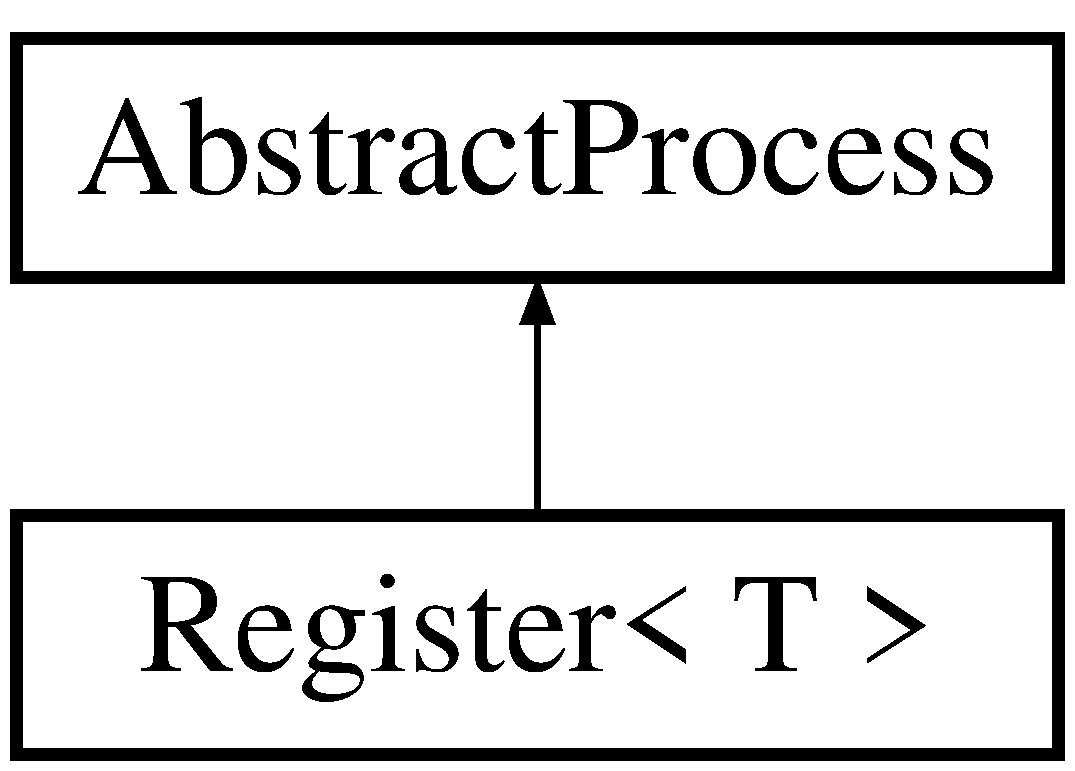
\includegraphics[height=2.000000cm]{classAbstractProcess}
\end{center}
\end{figure}
\subsection*{Public Member Functions}
\begin{DoxyCompactItemize}
\item 
\mbox{\Hypertarget{classAbstractProcess_aca866d43e7fe7c162c49a216f6393a4d}\label{classAbstractProcess_aca866d43e7fe7c162c49a216f6393a4d}} 
\mbox{\hyperlink{classAbstractProcess_aca866d43e7fe7c162c49a216f6393a4d}{Abstract\+Process}} ()
\begin{DoxyCompactList}\small\item\em Constructor. \end{DoxyCompactList}\item 
\mbox{\Hypertarget{classAbstractProcess_a9ae2142671945c6d92724d2daa5172cb}\label{classAbstractProcess_a9ae2142671945c6d92724d2daa5172cb}} 
virtual \mbox{\hyperlink{classAbstractProcess_a9ae2142671945c6d92724d2daa5172cb}{$\sim$\+Abstract\+Process}} ()
\begin{DoxyCompactList}\small\item\em Destructor. \end{DoxyCompactList}\item 
\mbox{\Hypertarget{classAbstractProcess_a8774aa41d5859b559b78e89cc48a65f0}\label{classAbstractProcess_a8774aa41d5859b559b78e89cc48a65f0}} 
virtual \mbox{\hyperlink{classMicroProcesses_1_1Process}{Micro\+Processes\+::\+Process}} $\ast$ \mbox{\hyperlink{classAbstractProcess_a8774aa41d5859b559b78e89cc48a65f0}{create}} ()=0
\begin{DoxyCompactList}\small\item\em Pure virtual method for creating a process. \end{DoxyCompactList}\end{DoxyCompactItemize}


\subsection{Detailed Description}
The abstract class which is used for the process factory 

The documentation for this class was generated from the following file\+:\begin{DoxyCompactItemize}
\item 
abstract\+\_\+process.\+h\end{DoxyCompactItemize}

\hypertarget{classMicroProcesses_1_1Adsorption}{}\section{Micro\+Processes\+:\+:Adsorption Class Reference}
\label{classMicroProcesses_1_1Adsorption}\index{Micro\+Processes\+::\+Adsorption@{Micro\+Processes\+::\+Adsorption}}


{\ttfamily \#include $<$adsorption.\+h$>$}

Inheritance diagram for Micro\+Processes\+:\+:Adsorption\+:\begin{figure}[H]
\begin{center}
\leavevmode
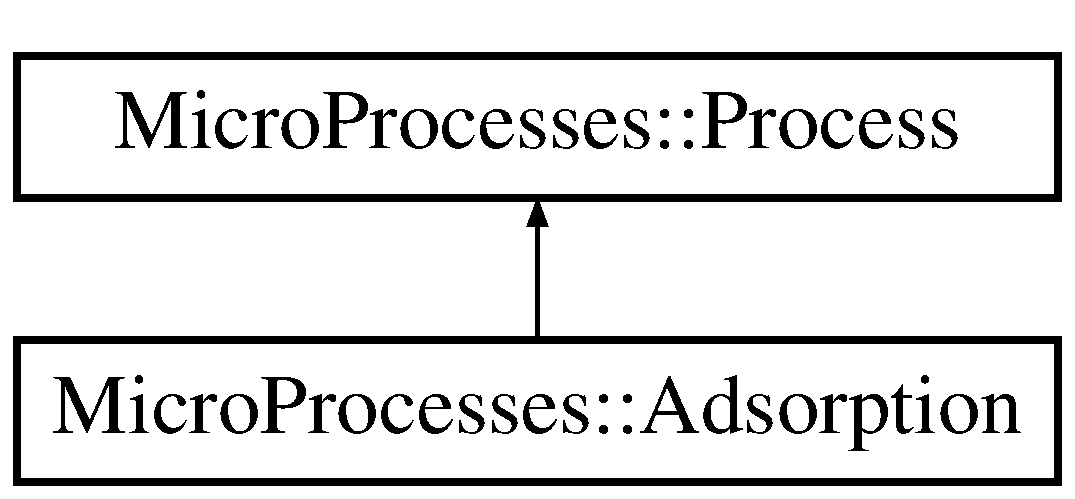
\includegraphics[height=2.000000cm]{classMicroProcesses_1_1Adsorption}
\end{center}
\end{figure}
\subsection*{Public Member Functions}
\begin{DoxyCompactItemize}
\item 
\mbox{\Hypertarget{classMicroProcesses_1_1Adsorption_a97591e8501cd748e11fcb863f030151f}\label{classMicroProcesses_1_1Adsorption_a97591e8501cd748e11fcb863f030151f}} 
\mbox{\hyperlink{classMicroProcesses_1_1Adsorption_a97591e8501cd748e11fcb863f030151f}{Adsorption}} ()
\begin{DoxyCompactList}\small\item\em Constructor. \end{DoxyCompactList}\item 
\mbox{\Hypertarget{classMicroProcesses_1_1Adsorption_a711c074d39b4fe218bb9229fb42bb4e3}\label{classMicroProcesses_1_1Adsorption_a711c074d39b4fe218bb9229fb42bb4e3}} 
virtual \mbox{\hyperlink{classMicroProcesses_1_1Adsorption_a711c074d39b4fe218bb9229fb42bb4e3}{$\sim$\+Adsorption}} ()
\begin{DoxyCompactList}\small\item\em Destructor. \end{DoxyCompactList}\item 
\mbox{\Hypertarget{classMicroProcesses_1_1Adsorption_ac0488825b7514a0866f52996730ad407}\label{classMicroProcesses_1_1Adsorption_ac0488825b7514a0866f52996730ad407}} 
void \mbox{\hyperlink{classMicroProcesses_1_1Adsorption_ac0488825b7514a0866f52996730ad407}{init}} ()
\begin{DoxyCompactList}\small\item\em Here everyhing needed for initialization of the process should be put. \end{DoxyCompactList}\item 
\mbox{\Hypertarget{classMicroProcesses_1_1Adsorption_ab0382497dbd736345c80a301c069455d}\label{classMicroProcesses_1_1Adsorption_ab0382497dbd736345c80a301c069455d}} 
void \mbox{\hyperlink{classMicroProcesses_1_1Adsorption_ab0382497dbd736345c80a301c069455d}{set\+Name}} (string s)
\begin{DoxyCompactList}\small\item\em The name of the process. \end{DoxyCompactList}\item 
\mbox{\Hypertarget{classMicroProcesses_1_1Adsorption_a7bc570bc528b5a8903556dc7f9b2c681}\label{classMicroProcesses_1_1Adsorption_a7bc570bc528b5a8903556dc7f9b2c681}} 
double \mbox{\hyperlink{classMicroProcesses_1_1Adsorption_a7bc570bc528b5a8903556dc7f9b2c681}{get\+Probability}} ()
\begin{DoxyCompactList}\small\item\em Compute the overall probabilities of this process and return it. \end{DoxyCompactList}\item 
\mbox{\Hypertarget{classMicroProcesses_1_1Adsorption_a1c94a7d3b64f9c60ae72879ef0b50cc2}\label{classMicroProcesses_1_1Adsorption_a1c94a7d3b64f9c60ae72879ef0b50cc2}} 
string \mbox{\hyperlink{classMicroProcesses_1_1Adsorption_a1c94a7d3b64f9c60ae72879ef0b50cc2}{get\+Name}} ()
\begin{DoxyCompactList}\small\item\em Returns the name of the process. \end{DoxyCompactList}\item 
void \mbox{\hyperlink{classMicroProcesses_1_1Adsorption_a5faf57ecabf9d2de92d4e630593771d3}{set\+Instance}} (\mbox{\hyperlink{classApothesis}{Apothesis}} $\ast$apothesis)
\item 
\mbox{\Hypertarget{classMicroProcesses_1_1Adsorption_a42e317856d4e97770d456bf9568cb73d}\label{classMicroProcesses_1_1Adsorption_a42e317856d4e97770d456bf9568cb73d}} 
void \mbox{\hyperlink{classMicroProcesses_1_1Adsorption_a42e317856d4e97770d456bf9568cb73d}{active\+Sites}} (\mbox{\hyperlink{classLattice}{Lattice}} $\ast$)
\begin{DoxyCompactList}\small\item\em Constructs the sites that adsorption can be performed. \end{DoxyCompactList}\item 
\mbox{\Hypertarget{classMicroProcesses_1_1Adsorption_af20402b5bfbc7b627ad8de13bdc2c541}\label{classMicroProcesses_1_1Adsorption_af20402b5bfbc7b627ad8de13bdc2c541}} 
void \mbox{\hyperlink{classMicroProcesses_1_1Adsorption_af20402b5bfbc7b627ad8de13bdc2c541}{select\+Site}} ()
\begin{DoxyCompactList}\small\item\em Slect the site that the adsorption will be performed from the available sites. \end{DoxyCompactList}\item 
\mbox{\Hypertarget{classMicroProcesses_1_1Adsorption_af67f833e6d63a35ac7c619997350e24c}\label{classMicroProcesses_1_1Adsorption_af67f833e6d63a35ac7c619997350e24c}} 
void \mbox{\hyperlink{classMicroProcesses_1_1Adsorption_af67f833e6d63a35ac7c619997350e24c}{perform}} ()
\begin{DoxyCompactList}\small\item\em Perform the process. This is what actually is called by the main K\+MC instance. \end{DoxyCompactList}\item 
void \mbox{\hyperlink{classMicroProcesses_1_1Adsorption_ab64c4f96f4b1b612db57c90c82140e3b}{set\+Process\+Map}} (map$<$ \mbox{\hyperlink{classMicroProcesses_1_1Process}{Process}} $\ast$, list$<$ \mbox{\hyperlink{classSurfaceTiles_1_1Site}{Site}} $\ast$ $>$ $\ast$ $>$ $\ast$)
\item 
\mbox{\Hypertarget{classMicroProcesses_1_1Adsorption_ac8bab3e2a04a6ea204c8f31077fb83fb}\label{classMicroProcesses_1_1Adsorption_ac8bab3e2a04a6ea204c8f31077fb83fb}} 
list$<$ \mbox{\hyperlink{classSurfaceTiles_1_1Site}{Site}} $\ast$ $>$ \mbox{\hyperlink{classMicroProcesses_1_1Adsorption_ac8bab3e2a04a6ea204c8f31077fb83fb}{get\+Active\+List}} ()
\begin{DoxyCompactList}\small\item\em The list of active sites for adsorption. \end{DoxyCompactList}\item 
void \mbox{\hyperlink{classMicroProcesses_1_1Adsorption_a891d1db6714ecbe9c3f698febc376652}{test}} ()
\item 
\mbox{\Hypertarget{classMicroProcesses_1_1Adsorption_ae234d5e6fe93a898dc5893a55117a34a}\label{classMicroProcesses_1_1Adsorption_ae234d5e6fe93a898dc5893a55117a34a}} 
bool \mbox{\hyperlink{classMicroProcesses_1_1Adsorption_ae234d5e6fe93a898dc5893a55117a34a}{controlt\+Rules}} (\mbox{\hyperlink{classSurfaceTiles_1_1Site}{Site}} $\ast$site)
\begin{DoxyCompactList}\small\item\em Returns true if the process can be performed in the site that callls it. \end{DoxyCompactList}\end{DoxyCompactItemize}
\subsection*{Protected Member Functions}
\begin{DoxyCompactItemize}
\item 
\mbox{\Hypertarget{classMicroProcesses_1_1Adsorption_a9c807426af10a4f2ff89abf7d774307f}\label{classMicroProcesses_1_1Adsorption_a9c807426af10a4f2ff89abf7d774307f}} 
void \mbox{\hyperlink{classMicroProcesses_1_1Adsorption_a9c807426af10a4f2ff89abf7d774307f}{mf\+\_\+remove\+From\+List}} ()
\begin{DoxyCompactList}\small\item\em Remove a site from a list. \end{DoxyCompactList}\item 
\mbox{\Hypertarget{classMicroProcesses_1_1Adsorption_a0bef9ba6310dcd4fece5add56e3cacfb}\label{classMicroProcesses_1_1Adsorption_a0bef9ba6310dcd4fece5add56e3cacfb}} 
void \mbox{\hyperlink{classMicroProcesses_1_1Adsorption_a0bef9ba6310dcd4fece5add56e3cacfb}{mf\+\_\+add\+To\+List}} (\mbox{\hyperlink{classSurfaceTiles_1_1Site}{Site}} $\ast$s)
\begin{DoxyCompactList}\small\item\em Add a site to a list. \end{DoxyCompactList}\item 
void \mbox{\hyperlink{classMicroProcesses_1_1Adsorption_a21cf31bffb1e123fb683c6f0c76b8717}{mf\+\_\+update\+Neigh\+Num}} ()
\end{DoxyCompactItemize}
\subsection*{Protected Attributes}
\begin{DoxyCompactItemize}
\item 
\mbox{\Hypertarget{classMicroProcesses_1_1Adsorption_af6e9c1e66d6123567c7067d1ae437b4f}\label{classMicroProcesses_1_1Adsorption_af6e9c1e66d6123567c7067d1ae437b4f}} 
\mbox{\hyperlink{classApothesis}{Apothesis}} $\ast$ \mbox{\hyperlink{classMicroProcesses_1_1Adsorption_af6e9c1e66d6123567c7067d1ae437b4f}{m\+\_\+apothesis}}
\begin{DoxyCompactList}\small\item\em The kmc instance. \end{DoxyCompactList}\item 
\mbox{\Hypertarget{classMicroProcesses_1_1Adsorption_a126b71d293e9dd6c9c8642777b964dad}\label{classMicroProcesses_1_1Adsorption_a126b71d293e9dd6c9c8642777b964dad}} 
string \mbox{\hyperlink{classMicroProcesses_1_1Adsorption_a126b71d293e9dd6c9c8642777b964dad}{m\+\_\+s\+Name}}
\begin{DoxyCompactList}\small\item\em The name of the process. \end{DoxyCompactList}\item 
\mbox{\Hypertarget{classMicroProcesses_1_1Adsorption_a7860184cf3917fe62a8e137a44faf6f2}\label{classMicroProcesses_1_1Adsorption_a7860184cf3917fe62a8e137a44faf6f2}} 
\mbox{\hyperlink{classSurfaceTiles_1_1Site}{Site}} $\ast$ \mbox{\hyperlink{classMicroProcesses_1_1Adsorption_a7860184cf3917fe62a8e137a44faf6f2}{m\+\_\+site}}
\begin{DoxyCompactList}\small\item\em The site that adsorption is performed. \end{DoxyCompactList}\item 
\mbox{\Hypertarget{classMicroProcesses_1_1Adsorption_a5c969a024e7decd889faee819af27bbc}\label{classMicroProcesses_1_1Adsorption_a5c969a024e7decd889faee819af27bbc}} 
double \mbox{\hyperlink{classMicroProcesses_1_1Adsorption_a5c969a024e7decd889faee819af27bbc}{m\+\_\+d\+Probability}}
\begin{DoxyCompactList}\small\item\em The value of the probability of the process is stored here. \end{DoxyCompactList}\item 
\mbox{\Hypertarget{classMicroProcesses_1_1Adsorption_a8d04e6d6ae56964fd9db536e4926bb42}\label{classMicroProcesses_1_1Adsorption_a8d04e6d6ae56964fd9db536e4926bb42}} 
int \mbox{\hyperlink{classMicroProcesses_1_1Adsorption_a8d04e6d6ae56964fd9db536e4926bb42}{m\+\_\+i\+Neigh\+Num}}
\begin{DoxyCompactList}\small\item\em The number of neighs of this site. \end{DoxyCompactList}\end{DoxyCompactItemize}


\subsection{Detailed Description}
The adsorption class. Adsoprtion depending on the type of lattice can be performed in different sites. For the simplest case e.\+g. B\+CC lattices all the sites are available for deposition. 

\subsection{Member Function Documentation}
\mbox{\Hypertarget{classMicroProcesses_1_1Adsorption_a21cf31bffb1e123fb683c6f0c76b8717}\label{classMicroProcesses_1_1Adsorption_a21cf31bffb1e123fb683c6f0c76b8717}} 
\index{Micro\+Processes\+::\+Adsorption@{Micro\+Processes\+::\+Adsorption}!mf\+\_\+update\+Neigh\+Num@{mf\+\_\+update\+Neigh\+Num}}
\index{mf\+\_\+update\+Neigh\+Num@{mf\+\_\+update\+Neigh\+Num}!Micro\+Processes\+::\+Adsorption@{Micro\+Processes\+::\+Adsorption}}
\subsubsection{\texorpdfstring{mf\+\_\+update\+Neigh\+Num()}{mf\_updateNeighNum()}}
{\footnotesize\ttfamily void Micro\+Processes\+::\+Adsorption\+::mf\+\_\+update\+Neigh\+Num (\begin{DoxyParamCaption}{ }\end{DoxyParamCaption})\hspace{0.3cm}{\ttfamily [protected]}}

Update the neighbour sites of this site. This is performed here since depending on the process this changes. E.\+g. fotr adsortpion in a F\+CC lattice the first neighbors are different compared to the adsroption in a B\+CC lattice. \mbox{\Hypertarget{classMicroProcesses_1_1Adsorption_a5faf57ecabf9d2de92d4e630593771d3}\label{classMicroProcesses_1_1Adsorption_a5faf57ecabf9d2de92d4e630593771d3}} 
\index{Micro\+Processes\+::\+Adsorption@{Micro\+Processes\+::\+Adsorption}!set\+Instance@{set\+Instance}}
\index{set\+Instance@{set\+Instance}!Micro\+Processes\+::\+Adsorption@{Micro\+Processes\+::\+Adsorption}}
\subsubsection{\texorpdfstring{set\+Instance()}{setInstance()}}
{\footnotesize\ttfamily void Micro\+Processes\+::\+Adsorption\+::set\+Instance (\begin{DoxyParamCaption}\item[{\mbox{\hyperlink{classApothesis}{Apothesis}} $\ast$}]{apothesis }\end{DoxyParamCaption})\hspace{0.3cm}{\ttfamily [inline]}, {\ttfamily [virtual]}}

Set the instance of the kmc. This allows to have access to all other functionalities of the K\+MC class. 

Implements \mbox{\hyperlink{classMicroProcesses_1_1Process_a4c419af2e6e6477200b45bf687783c84}{Micro\+Processes\+::\+Process}}.

\mbox{\Hypertarget{classMicroProcesses_1_1Adsorption_ab64c4f96f4b1b612db57c90c82140e3b}\label{classMicroProcesses_1_1Adsorption_ab64c4f96f4b1b612db57c90c82140e3b}} 
\index{Micro\+Processes\+::\+Adsorption@{Micro\+Processes\+::\+Adsorption}!set\+Process\+Map@{set\+Process\+Map}}
\index{set\+Process\+Map@{set\+Process\+Map}!Micro\+Processes\+::\+Adsorption@{Micro\+Processes\+::\+Adsorption}}
\subsubsection{\texorpdfstring{set\+Process\+Map()}{setProcessMap()}}
{\footnotesize\ttfamily void Micro\+Processes\+::\+Adsorption\+::set\+Process\+Map (\begin{DoxyParamCaption}\item[{map$<$ \mbox{\hyperlink{classMicroProcesses_1_1Process}{Process}} $\ast$, list$<$ \mbox{\hyperlink{classSurfaceTiles_1_1Site}{Site}} $\ast$ $>$ $\ast$ $>$ $\ast$}]{proc\+Map }\end{DoxyParamCaption})\hspace{0.3cm}{\ttfamily [virtual]}}

A process map which is used between the different processes. This need to be evaluated since it is not so handy. 

Implements \mbox{\hyperlink{classMicroProcesses_1_1Process_a4e726f7491eb805efd9dcd1c0c3a380f}{Micro\+Processes\+::\+Process}}.

\mbox{\Hypertarget{classMicroProcesses_1_1Adsorption_a891d1db6714ecbe9c3f698febc376652}\label{classMicroProcesses_1_1Adsorption_a891d1db6714ecbe9c3f698febc376652}} 
\index{Micro\+Processes\+::\+Adsorption@{Micro\+Processes\+::\+Adsorption}!test@{test}}
\index{test@{test}!Micro\+Processes\+::\+Adsorption@{Micro\+Processes\+::\+Adsorption}}
\subsubsection{\texorpdfstring{test()}{test()}}
{\footnotesize\ttfamily void Micro\+Processes\+::\+Adsorption\+::test (\begin{DoxyParamCaption}{ }\end{DoxyParamCaption})}

Here various tests should be putted in order to check for the validity of the process e.\+g. the number of the particles in the active surface must be constant (mass is constant). 

The documentation for this class was generated from the following files\+:\begin{DoxyCompactItemize}
\item 
adsorption.\+h\item 
adsorption.\+cpp\end{DoxyCompactItemize}

\hypertarget{classApothesis}{}\section{Apothesis Class Reference}
\label{classApothesis}\index{Apothesis@{Apothesis}}
\subsection*{Public Member Functions}
\begin{DoxyCompactItemize}
\item 
\mbox{\Hypertarget{classApothesis_a7977d54d81e24129bfacdd142fc8695f}\label{classApothesis_a7977d54d81e24129bfacdd142fc8695f}} 
{\bfseries Apothesis} (int argc, char $\ast$argv\mbox{[}$\,$\mbox{]})
\item 
void \mbox{\hyperlink{classApothesis_acef1e97b07815dbc4879c28521b856ab}{init}} ()
\item 
void \mbox{\hyperlink{classApothesis_a423ade721d6955058ceca935908bada0}{exec}} ()
\begin{DoxyCompactList}\small\item\em Perform the K\+MC iteratios. \end{DoxyCompactList}\end{DoxyCompactItemize}
\subsection*{Public Attributes}
\begin{DoxyCompactItemize}
\item 
\mbox{\hyperlink{classIO}{IO}} $\ast$ \mbox{\hyperlink{classApothesis_a9b445e59759acb31785cec5412ae1fe4}{p\+IO}}
\begin{DoxyCompactList}\small\item\em \mbox{\hyperlink{classPointers}{Pointers}} to the classes that will share the common space i.\+e. the \char`\"{}pointer\char`\"{}. \end{DoxyCompactList}\item 
\mbox{\Hypertarget{classApothesis_abfdba0ca793f52cbed2b6de31083d3c2}\label{classApothesis_abfdba0ca793f52cbed2b6de31083d3c2}} 
\mbox{\hyperlink{classLattice}{Lattice}} $\ast$ \mbox{\hyperlink{classApothesis_abfdba0ca793f52cbed2b6de31083d3c2}{p\+Lattice}}
\begin{DoxyCompactList}\small\item\em Pointer to the lattice class. \end{DoxyCompactList}\item 
\mbox{\Hypertarget{classApothesis_a37927f2ba90323bc6da8f3eecee9400e}\label{classApothesis_a37927f2ba90323bc6da8f3eecee9400e}} 
\mbox{\hyperlink{classUtils_1_1ErrorHandler}{Utils\+::\+Error\+Handler}} $\ast$ \mbox{\hyperlink{classApothesis_a37927f2ba90323bc6da8f3eecee9400e}{p\+Error\+Handler}}
\begin{DoxyCompactList}\small\item\em Pointer to the error class. \end{DoxyCompactList}\item 
\mbox{\Hypertarget{classApothesis_aef7a188e3e674cc0160e8bd3425ef669}\label{classApothesis_aef7a188e3e674cc0160e8bd3425ef669}} 
\mbox{\hyperlink{classUtils_1_1Parameters}{Utils\+::\+Parameters}} $\ast$ \mbox{\hyperlink{classApothesis_aef7a188e3e674cc0160e8bd3425ef669}{p\+Parameters}}
\begin{DoxyCompactList}\small\item\em Pointer to the paramters class. \end{DoxyCompactList}\end{DoxyCompactItemize}


\subsection{Member Function Documentation}
\mbox{\Hypertarget{classApothesis_a423ade721d6955058ceca935908bada0}\label{classApothesis_a423ade721d6955058ceca935908bada0}} 
\index{Apothesis@{Apothesis}!exec@{exec}}
\index{exec@{exec}!Apothesis@{Apothesis}}
\subsubsection{\texorpdfstring{exec()}{exec()}}
{\footnotesize\ttfamily void Apothesis\+::exec (\begin{DoxyParamCaption}{ }\end{DoxyParamCaption})}



Perform the K\+MC iteratios. 

Perform the number of K\+MC steps read from the input.

Here a process should be selected in random. We have only one for now...

Print to output

Get the active sites of the process

Check if there are available sites that it can be performed

Select randomly a site

Perform the process

The frequency that the various information are written in the file must befined by the user. Fix it ... The user should also check if the messages are written on the terminal or not. \mbox{\Hypertarget{classApothesis_acef1e97b07815dbc4879c28521b856ab}\label{classApothesis_acef1e97b07815dbc4879c28521b856ab}} 
\index{Apothesis@{Apothesis}!init@{init}}
\index{init@{init}!Apothesis@{Apothesis}}
\subsubsection{\texorpdfstring{init()}{init()}}
{\footnotesize\ttfamily void Apothesis\+::init (\begin{DoxyParamCaption}{ }\end{DoxyParamCaption})}

Intialization of the K\+MC method. For example here the processes to be performed as these are written in the input file are constcucted through the factory method Get the processes read and create them

The output file name will come from the user and will have the extenstion .log This would come as a parameter from the user from the args (also the input). Now both are hard copied. ~\newline
 First the processes that participate in the simulation that were read from the file input and the I/O functionality 

\subsection{Member Data Documentation}
\mbox{\Hypertarget{classApothesis_a9b445e59759acb31785cec5412ae1fe4}\label{classApothesis_a9b445e59759acb31785cec5412ae1fe4}} 
\index{Apothesis@{Apothesis}!p\+IO@{p\+IO}}
\index{p\+IO@{p\+IO}!Apothesis@{Apothesis}}
\subsubsection{\texorpdfstring{p\+IO}{pIO}}
{\footnotesize\ttfamily \mbox{\hyperlink{classIO}{IO}}$\ast$ Apothesis\+::p\+IO}



\mbox{\hyperlink{classPointers}{Pointers}} to the classes that will share the common space i.\+e. the \char`\"{}pointer\char`\"{}. 

Ponter to the input/output class 

The documentation for this class was generated from the following files\+:\begin{DoxyCompactItemize}
\item 
apothesis.\+h\item 
apothesis.\+cpp\end{DoxyCompactItemize}

\hypertarget{classMicroProcesses_1_1Diffusion}{}\section{Micro\+Processes\+:\+:Diffusion Class Reference}
\label{classMicroProcesses_1_1Diffusion}\index{Micro\+Processes\+::\+Diffusion@{Micro\+Processes\+::\+Diffusion}}
Inheritance diagram for Micro\+Processes\+:\+:Diffusion\+:\begin{figure}[H]
\begin{center}
\leavevmode
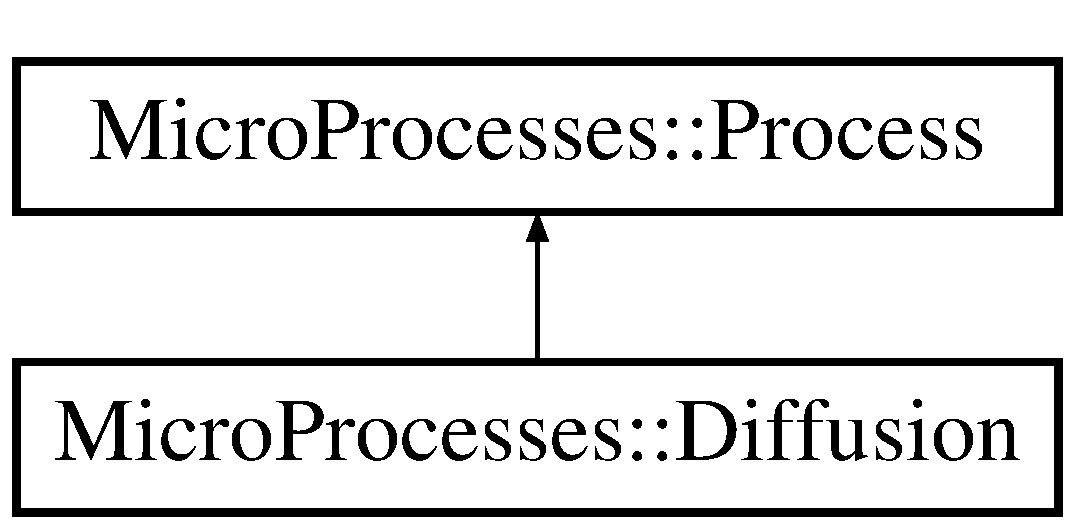
\includegraphics[height=2.000000cm]{classMicroProcesses_1_1Diffusion}
\end{center}
\end{figure}
\subsection*{Public Member Functions}
\begin{DoxyCompactItemize}
\item 
\mbox{\Hypertarget{classMicroProcesses_1_1Diffusion_ac9ea5351a9030303907c2bf866076aa2}\label{classMicroProcesses_1_1Diffusion_ac9ea5351a9030303907c2bf866076aa2}} 
\mbox{\hyperlink{classMicroProcesses_1_1Diffusion_ac9ea5351a9030303907c2bf866076aa2}{Diffusion}} ()
\begin{DoxyCompactList}\small\item\em Constructor. \end{DoxyCompactList}\item 
\mbox{\Hypertarget{classMicroProcesses_1_1Diffusion_ad8f0097d8ef4e20a5e4c4e6a2bc0c228}\label{classMicroProcesses_1_1Diffusion_ad8f0097d8ef4e20a5e4c4e6a2bc0c228}} 
virtual \mbox{\hyperlink{classMicroProcesses_1_1Diffusion_ad8f0097d8ef4e20a5e4c4e6a2bc0c228}{$\sim$\+Diffusion}} ()
\begin{DoxyCompactList}\small\item\em Destructor. \end{DoxyCompactList}\item 
\mbox{\Hypertarget{classMicroProcesses_1_1Diffusion_abdf4a0708fdec9bc6877418afaf51bb5}\label{classMicroProcesses_1_1Diffusion_abdf4a0708fdec9bc6877418afaf51bb5}} 
void \mbox{\hyperlink{classMicroProcesses_1_1Diffusion_abdf4a0708fdec9bc6877418afaf51bb5}{init}} ()
\begin{DoxyCompactList}\small\item\em Here everyhing needed for initialization of the process should be put. \end{DoxyCompactList}\item 
\mbox{\Hypertarget{classMicroProcesses_1_1Diffusion_a8828bfcf075bd04443de9e9932fb5eab}\label{classMicroProcesses_1_1Diffusion_a8828bfcf075bd04443de9e9932fb5eab}} 
void \mbox{\hyperlink{classMicroProcesses_1_1Diffusion_a8828bfcf075bd04443de9e9932fb5eab}{set\+Name}} (string s)
\begin{DoxyCompactList}\small\item\em The name of the process. \end{DoxyCompactList}\item 
\mbox{\Hypertarget{classMicroProcesses_1_1Diffusion_af483d53a291f3524a273d35d24f7f24c}\label{classMicroProcesses_1_1Diffusion_af483d53a291f3524a273d35d24f7f24c}} 
double \mbox{\hyperlink{classMicroProcesses_1_1Diffusion_af483d53a291f3524a273d35d24f7f24c}{get\+Probability}} ()
\begin{DoxyCompactList}\small\item\em Compute the overall probabilities of this process and return it. \end{DoxyCompactList}\item 
\mbox{\Hypertarget{classMicroProcesses_1_1Diffusion_ad6cab95e42f11fed711a7b7b324291c8}\label{classMicroProcesses_1_1Diffusion_ad6cab95e42f11fed711a7b7b324291c8}} 
string \mbox{\hyperlink{classMicroProcesses_1_1Diffusion_ad6cab95e42f11fed711a7b7b324291c8}{get\+Name}} ()
\begin{DoxyCompactList}\small\item\em Returns the name of the process. \end{DoxyCompactList}\item 
void \mbox{\hyperlink{classMicroProcesses_1_1Diffusion_a17993edabb08ca2fb96d22ef3cd838ca}{set\+Instance}} (\mbox{\hyperlink{classApothesis}{Apothesis}} $\ast$apothesis)
\item 
\mbox{\Hypertarget{classMicroProcesses_1_1Diffusion_ad82f57afa447a4d96b596d242ffb67e2}\label{classMicroProcesses_1_1Diffusion_ad82f57afa447a4d96b596d242ffb67e2}} 
void \mbox{\hyperlink{classMicroProcesses_1_1Diffusion_ad82f57afa447a4d96b596d242ffb67e2}{active\+Sites}} (\mbox{\hyperlink{classLattice}{Lattice}} $\ast$)
\begin{DoxyCompactList}\small\item\em Set the lattice uppon which adsorpiton will be performed. \end{DoxyCompactList}\item 
\mbox{\Hypertarget{classMicroProcesses_1_1Diffusion_af699c30b1c182cce03e9a9826b0c5b51}\label{classMicroProcesses_1_1Diffusion_af699c30b1c182cce03e9a9826b0c5b51}} 
void \mbox{\hyperlink{classMicroProcesses_1_1Diffusion_af699c30b1c182cce03e9a9826b0c5b51}{select\+Site}} ()
\begin{DoxyCompactList}\small\item\em The initial site that the diffusion will begin. \end{DoxyCompactList}\item 
\mbox{\Hypertarget{classMicroProcesses_1_1Diffusion_afff30436b63d3842c87895358ddbd575}\label{classMicroProcesses_1_1Diffusion_afff30436b63d3842c87895358ddbd575}} 
void \mbox{\hyperlink{classMicroProcesses_1_1Diffusion_afff30436b63d3842c87895358ddbd575}{perform}} ()
\begin{DoxyCompactList}\small\item\em Perform the process. This is what actually is called by the main K\+MC instance. \end{DoxyCompactList}\item 
void \mbox{\hyperlink{classMicroProcesses_1_1Diffusion_a53e5d56710045b4f8783d9c05591357f}{set\+Process\+Map}} (map$<$ \mbox{\hyperlink{classMicroProcesses_1_1Process}{Process}} $\ast$, list$<$ \mbox{\hyperlink{classSurfaceTiles_1_1Site}{Site}} $\ast$ $>$ $\ast$ $>$ $\ast$)
\item 
\mbox{\Hypertarget{classMicroProcesses_1_1Diffusion_a8e19130f8f9948f1a6a446f4065027dd}\label{classMicroProcesses_1_1Diffusion_a8e19130f8f9948f1a6a446f4065027dd}} 
list$<$ \mbox{\hyperlink{classSurfaceTiles_1_1Site}{Site}} $\ast$$>$ \mbox{\hyperlink{classMicroProcesses_1_1Diffusion_a8e19130f8f9948f1a6a446f4065027dd}{get\+Active\+List}} ()
\begin{DoxyCompactList}\small\item\em The list of active sites for diffusion. \end{DoxyCompactList}\item 
void \mbox{\hyperlink{classMicroProcesses_1_1Diffusion_a281afcddb42b87ae9ba3b48a54524cd1}{test}} ()
\end{DoxyCompactItemize}
\subsection*{Protected Attributes}
\begin{DoxyCompactItemize}
\item 
\mbox{\Hypertarget{classMicroProcesses_1_1Diffusion_aa5938a315954467db6f7d7f4e59fcf62}\label{classMicroProcesses_1_1Diffusion_aa5938a315954467db6f7d7f4e59fcf62}} 
\mbox{\hyperlink{classApothesis}{Apothesis}} $\ast$ \mbox{\hyperlink{classMicroProcesses_1_1Diffusion_aa5938a315954467db6f7d7f4e59fcf62}{m\+\_\+apothesis}}
\begin{DoxyCompactList}\small\item\em The kmc instance. \end{DoxyCompactList}\end{DoxyCompactItemize}


\subsection{Member Function Documentation}
\mbox{\Hypertarget{classMicroProcesses_1_1Diffusion_a17993edabb08ca2fb96d22ef3cd838ca}\label{classMicroProcesses_1_1Diffusion_a17993edabb08ca2fb96d22ef3cd838ca}} 
\index{Micro\+Processes\+::\+Diffusion@{Micro\+Processes\+::\+Diffusion}!set\+Instance@{set\+Instance}}
\index{set\+Instance@{set\+Instance}!Micro\+Processes\+::\+Diffusion@{Micro\+Processes\+::\+Diffusion}}
\subsubsection{\texorpdfstring{set\+Instance()}{setInstance()}}
{\footnotesize\ttfamily void Micro\+Processes\+::\+Diffusion\+::set\+Instance (\begin{DoxyParamCaption}\item[{\mbox{\hyperlink{classApothesis}{Apothesis}} $\ast$}]{apothesis }\end{DoxyParamCaption})\hspace{0.3cm}{\ttfamily [inline]}, {\ttfamily [virtual]}}

Set the instance of \mbox{\hyperlink{classApothesis}{Apothesis}}. This allows to have access to all other functionalities of the K\+MC class. 

Implements \mbox{\hyperlink{classMicroProcesses_1_1Process_a4c419af2e6e6477200b45bf687783c84}{Micro\+Processes\+::\+Process}}.

\mbox{\Hypertarget{classMicroProcesses_1_1Diffusion_a53e5d56710045b4f8783d9c05591357f}\label{classMicroProcesses_1_1Diffusion_a53e5d56710045b4f8783d9c05591357f}} 
\index{Micro\+Processes\+::\+Diffusion@{Micro\+Processes\+::\+Diffusion}!set\+Process\+Map@{set\+Process\+Map}}
\index{set\+Process\+Map@{set\+Process\+Map}!Micro\+Processes\+::\+Diffusion@{Micro\+Processes\+::\+Diffusion}}
\subsubsection{\texorpdfstring{set\+Process\+Map()}{setProcessMap()}}
{\footnotesize\ttfamily void Micro\+Processes\+::\+Diffusion\+::set\+Process\+Map (\begin{DoxyParamCaption}\item[{map$<$ \mbox{\hyperlink{classMicroProcesses_1_1Process}{Process}} $\ast$, list$<$ \mbox{\hyperlink{classSurfaceTiles_1_1Site}{Site}} $\ast$ $>$ $\ast$ $>$ $\ast$}]{ }\end{DoxyParamCaption})\hspace{0.3cm}{\ttfamily [virtual]}}

A process map which is used between the different processes. This need to be evaluated since it is not so handy. 

Implements \mbox{\hyperlink{classMicroProcesses_1_1Process_a4e726f7491eb805efd9dcd1c0c3a380f}{Micro\+Processes\+::\+Process}}.

\mbox{\Hypertarget{classMicroProcesses_1_1Diffusion_a281afcddb42b87ae9ba3b48a54524cd1}\label{classMicroProcesses_1_1Diffusion_a281afcddb42b87ae9ba3b48a54524cd1}} 
\index{Micro\+Processes\+::\+Diffusion@{Micro\+Processes\+::\+Diffusion}!test@{test}}
\index{test@{test}!Micro\+Processes\+::\+Diffusion@{Micro\+Processes\+::\+Diffusion}}
\subsubsection{\texorpdfstring{test()}{test()}}
{\footnotesize\ttfamily void Micro\+Processes\+::\+Diffusion\+::test (\begin{DoxyParamCaption}{ }\end{DoxyParamCaption})}

Here various tests should be putted in order to check for the validity of the process e.\+g. the number of the particles in the active surface must be constant (mass is constant). 

The documentation for this class was generated from the following files\+:\begin{DoxyCompactItemize}
\item 
diffusion.\+h\item 
diffusion.\+cpp\end{DoxyCompactItemize}

\hypertarget{classUtils_1_1ErrorHandler}{}\section{Utils\+:\+:Error\+Handler Class Reference}
\label{classUtils_1_1ErrorHandler}\index{Utils\+::\+Error\+Handler@{Utils\+::\+Error\+Handler}}


{\ttfamily \#include $<$errorhandler.\+h$>$}

Inheritance diagram for Utils\+:\+:Error\+Handler\+:\begin{figure}[H]
\begin{center}
\leavevmode
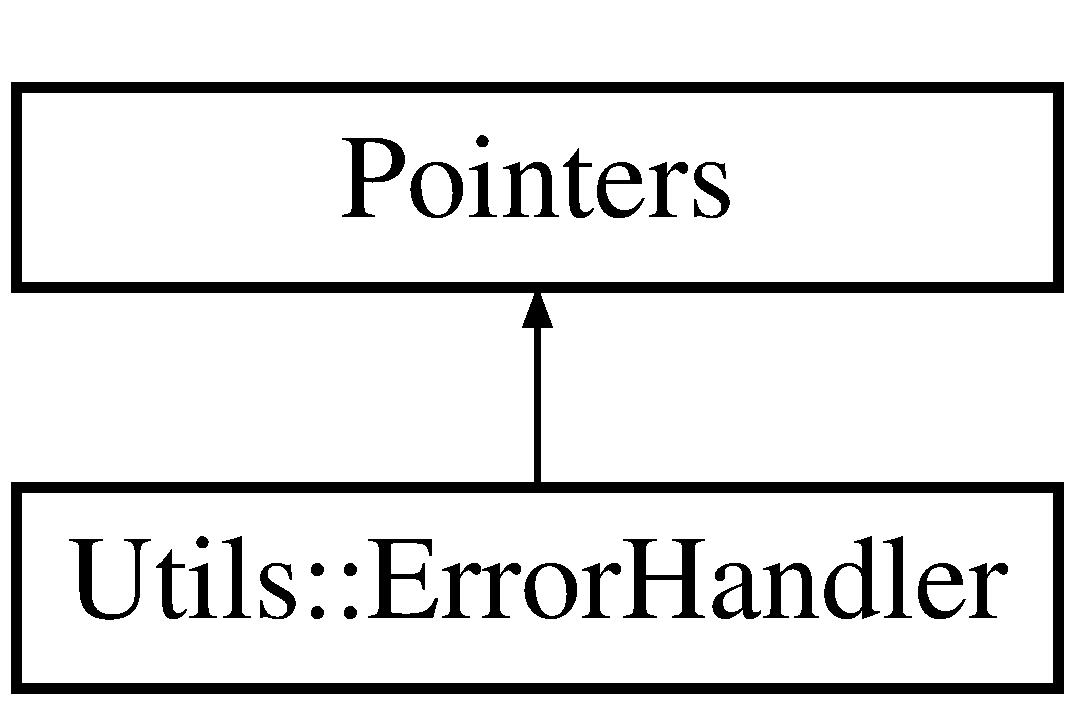
\includegraphics[height=2.000000cm]{classUtils_1_1ErrorHandler}
\end{center}
\end{figure}
\subsection*{Public Member Functions}
\begin{DoxyCompactItemize}
\item 
\mbox{\Hypertarget{classUtils_1_1ErrorHandler_af9d42cd68ec6959575b23f5e0acd1674}\label{classUtils_1_1ErrorHandler_af9d42cd68ec6959575b23f5e0acd1674}} 
\mbox{\hyperlink{classUtils_1_1ErrorHandler_af9d42cd68ec6959575b23f5e0acd1674}{Error\+Handler}} (\mbox{\hyperlink{classApothesis}{Apothesis}} $\ast$apothesis)
\begin{DoxyCompactList}\small\item\em Constructor. \end{DoxyCompactList}\item 
\mbox{\Hypertarget{classUtils_1_1ErrorHandler_ae9077e0d6ebdc00de2431b1fb83ee86f}\label{classUtils_1_1ErrorHandler_ae9077e0d6ebdc00de2431b1fb83ee86f}} 
virtual \mbox{\hyperlink{classUtils_1_1ErrorHandler_ae9077e0d6ebdc00de2431b1fb83ee86f}{$\sim$\+Error\+Handler}} ()
\begin{DoxyCompactList}\small\item\em Destructor. \end{DoxyCompactList}\item 
void \mbox{\hyperlink{classUtils_1_1ErrorHandler_a8b2b06323fcdb8e996104ff33cfc6840}{error\+\_\+simple\+\_\+msg}} (string msg)
\begin{DoxyCompactList}\small\item\em Different ways to handle an error depending on its nature. \end{DoxyCompactList}\item 
\mbox{\Hypertarget{classUtils_1_1ErrorHandler_a47765c6b3ec00dc1b17aeaa6c4e9a803}\label{classUtils_1_1ErrorHandler_a47765c6b3ec00dc1b17aeaa6c4e9a803}} 
void \mbox{\hyperlink{classUtils_1_1ErrorHandler_a47765c6b3ec00dc1b17aeaa6c4e9a803}{error\+Msg}} (const string \&file, const string \&filetype, int line, const string \&msg)
\begin{DoxyCompactList}\small\item\em Error message. \end{DoxyCompactList}\item 
\mbox{\Hypertarget{classUtils_1_1ErrorHandler_a05f868786277d5bbdc4707c36f122ba6}\label{classUtils_1_1ErrorHandler_a05f868786277d5bbdc4707c36f122ba6}} 
void \mbox{\hyperlink{classUtils_1_1ErrorHandler_a05f868786277d5bbdc4707c36f122ba6}{error\+Msg}} (const string \&file, const string \&filetype, int line, int column, const string \&msg)
\begin{DoxyCompactList}\small\item\em Error message. \end{DoxyCompactList}\item 
\mbox{\Hypertarget{classUtils_1_1ErrorHandler_a8f0a658e09dfcd13d3b075ff9080554f}\label{classUtils_1_1ErrorHandler_a8f0a658e09dfcd13d3b075ff9080554f}} 
void \mbox{\hyperlink{classUtils_1_1ErrorHandler_a8f0a658e09dfcd13d3b075ff9080554f}{error\+Msg}} (const string \&file, const string \&filetype, const string \&msg)
\begin{DoxyCompactList}\small\item\em Error message. \end{DoxyCompactList}\item 
\mbox{\Hypertarget{classUtils_1_1ErrorHandler_a42f8bebc7f7a9a80c7b763d82afe2074}\label{classUtils_1_1ErrorHandler_a42f8bebc7f7a9a80c7b763d82afe2074}} 
void \mbox{\hyperlink{classUtils_1_1ErrorHandler_a42f8bebc7f7a9a80c7b763d82afe2074}{warning\+Msg}} (const string \&file, const string \&filetype, const string \&msg)
\begin{DoxyCompactList}\small\item\em Warning message. \end{DoxyCompactList}\item 
\mbox{\Hypertarget{classUtils_1_1ErrorHandler_adb593ecfc758b7ddc5143e6a136bb53c}\label{classUtils_1_1ErrorHandler_adb593ecfc758b7ddc5143e6a136bb53c}} 
void \mbox{\hyperlink{classUtils_1_1ErrorHandler_adb593ecfc758b7ddc5143e6a136bb53c}{warning\+Msg}} (const string \&movetype, const string \&msg)
\begin{DoxyCompactList}\small\item\em Warning message. \end{DoxyCompactList}\item 
\mbox{\Hypertarget{classUtils_1_1ErrorHandler_afacf74c2bb2aefb55a2bf4efa561e92e}\label{classUtils_1_1ErrorHandler_afacf74c2bb2aefb55a2bf4efa561e92e}} 
void \mbox{\hyperlink{classUtils_1_1ErrorHandler_afacf74c2bb2aefb55a2bf4efa561e92e}{warning\+Simple\+\_\+msg}} (const string \&msg)
\begin{DoxyCompactList}\small\item\em Warning message simple text. \end{DoxyCompactList}\end{DoxyCompactItemize}
\subsection*{Additional Inherited Members}


\subsection{Detailed Description}
A class for handling the development and user errors. Different ways to handle an error depending on its nature. Many of the functions are not implememented yet. 

\subsection{Member Function Documentation}
\mbox{\Hypertarget{classUtils_1_1ErrorHandler_a8b2b06323fcdb8e996104ff33cfc6840}\label{classUtils_1_1ErrorHandler_a8b2b06323fcdb8e996104ff33cfc6840}} 
\index{Utils\+::\+Error\+Handler@{Utils\+::\+Error\+Handler}!error\+\_\+simple\+\_\+msg@{error\+\_\+simple\+\_\+msg}}
\index{error\+\_\+simple\+\_\+msg@{error\+\_\+simple\+\_\+msg}!Utils\+::\+Error\+Handler@{Utils\+::\+Error\+Handler}}
\subsubsection{\texorpdfstring{error\+\_\+simple\+\_\+msg()}{error\_simple\_msg()}}
{\footnotesize\ttfamily void Utils\+::\+Error\+Handler\+::error\+\_\+simple\+\_\+msg (\begin{DoxyParamCaption}\item[{string}]{msg }\end{DoxyParamCaption})}



Different ways to handle an error depending on its nature. 

Error message simple text 

The documentation for this class was generated from the following files\+:\begin{DoxyCompactItemize}
\item 
errorhandler.\+h\item 
errorhandler.\+cpp\end{DoxyCompactItemize}

\hypertarget{classFactoryProcess}{}\section{Factory\+Process Class Reference}
\label{classFactoryProcess}\index{Factory\+Process@{Factory\+Process}}
\subsection*{Public Member Functions}
\begin{DoxyCompactItemize}
\item 
\mbox{\Hypertarget{classFactoryProcess_a29186a501f70f12963785f4bcab4683a}\label{classFactoryProcess_a29186a501f70f12963785f4bcab4683a}} 
\mbox{\hyperlink{classFactoryProcess_a29186a501f70f12963785f4bcab4683a}{Factory\+Process}} ()
\begin{DoxyCompactList}\small\item\em Constructor. \end{DoxyCompactList}\item 
\mbox{\Hypertarget{classFactoryProcess_a9e1252dfb61df685d0fb2ba9e79d4a21}\label{classFactoryProcess_a9e1252dfb61df685d0fb2ba9e79d4a21}} 
virtual \mbox{\hyperlink{classFactoryProcess_a9e1252dfb61df685d0fb2ba9e79d4a21}{$\sim$\+Factory\+Process}} ()
\begin{DoxyCompactList}\small\item\em Destructor. \end{DoxyCompactList}\end{DoxyCompactItemize}
\subsection*{Static Public Member Functions}
\begin{DoxyCompactItemize}
\item 
\mbox{\Hypertarget{classFactoryProcess_a9621ffe953d445a0a2e4c6a3970c9b87}\label{classFactoryProcess_a9621ffe953d445a0a2e4c6a3970c9b87}} 
static void \mbox{\hyperlink{classFactoryProcess_a9621ffe953d445a0a2e4c6a3970c9b87}{register\+This}} (const string \&, \mbox{\hyperlink{classAbstractProcess}{Abstract\+Process}} $\ast$)
\begin{DoxyCompactList}\small\item\em \mbox{\hyperlink{classRegister}{Register}} the new process (Store it in the map table since a map table cannot be initialized) \end{DoxyCompactList}\item 
\mbox{\Hypertarget{classFactoryProcess_ae1d7d44a5e5ea56fdedf68f910f930ff}\label{classFactoryProcess_ae1d7d44a5e5ea56fdedf68f910f930ff}} 
static \mbox{\hyperlink{classMicroProcesses_1_1Process}{Micro\+Processes\+::\+Process}} $\ast$ \mbox{\hyperlink{classFactoryProcess_ae1d7d44a5e5ea56fdedf68f910f930ff}{create\+Process}} (const string \&)
\begin{DoxyCompactList}\small\item\em Create the process. \end{DoxyCompactList}\end{DoxyCompactItemize}


The documentation for this class was generated from the following files\+:\begin{DoxyCompactItemize}
\item 
factory\+\_\+process.\+h\item 
factory\+\_\+process.\+cpp\end{DoxyCompactItemize}

\hypertarget{classIO}{}\section{IO Class Reference}
\label{classIO}\index{IO@{IO}}


{\ttfamily \#include $<$io.\+h$>$}

Inheritance diagram for IO\+:\begin{figure}[H]
\begin{center}
\leavevmode
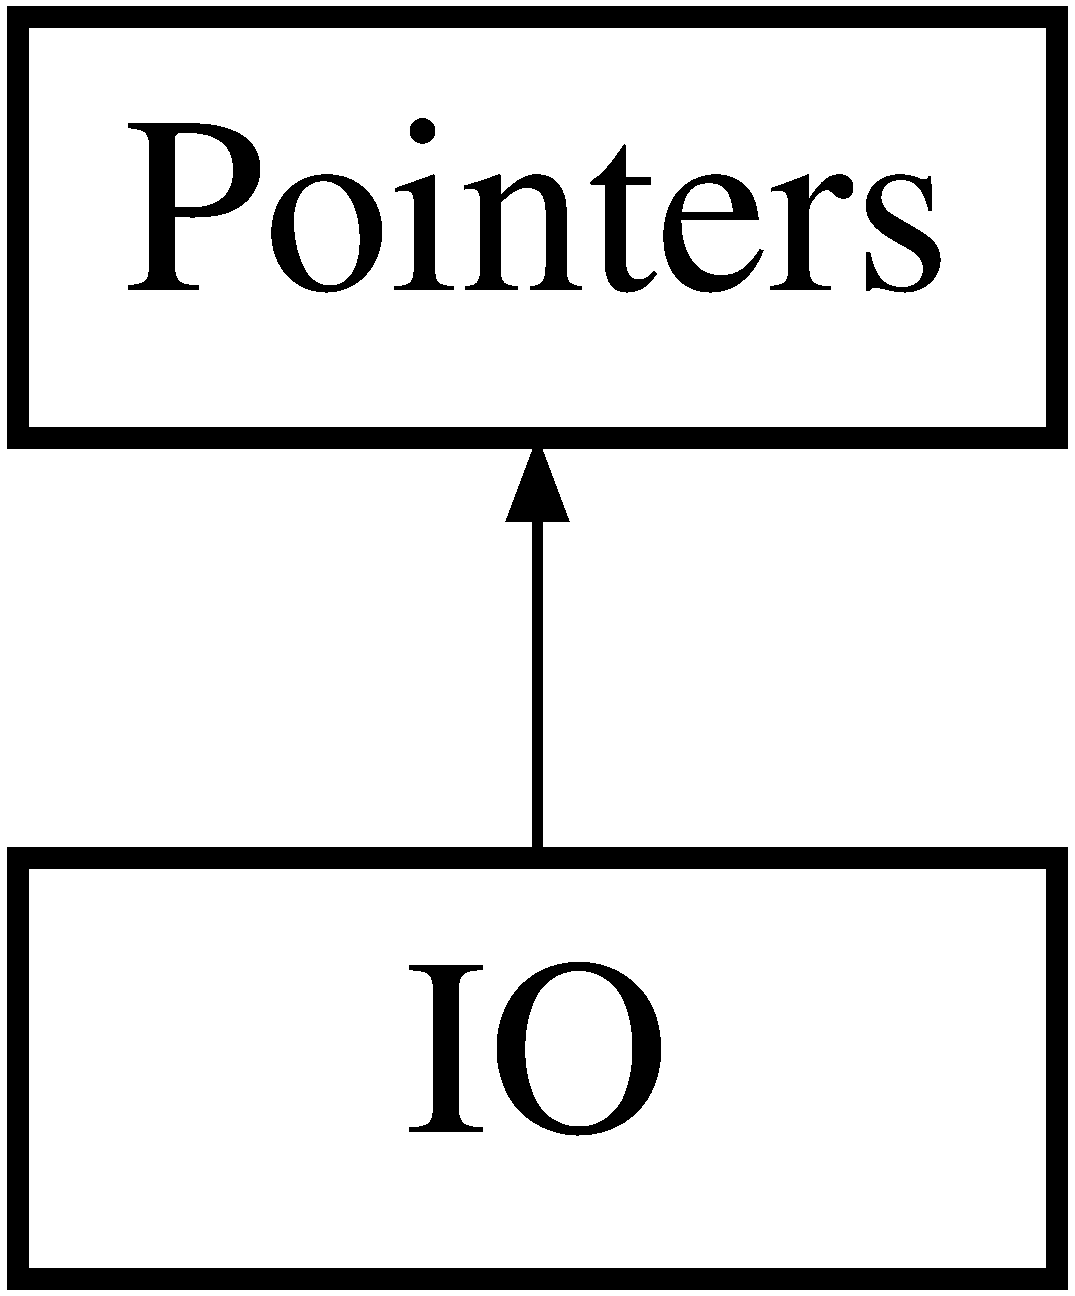
\includegraphics[height=2.000000cm]{classIO}
\end{center}
\end{figure}
\subsection*{Public Types}
\begin{DoxyCompactItemize}
\item 
\mbox{\Hypertarget{classIO_a527094b0734eedb3b151d65d5af39087}\label{classIO_a527094b0734eedb3b151d65d5af39087}} 
enum {\bfseries C\+A\+SE} \{ {\bfseries Sensitive}, 
{\bfseries Insensitive}
 \}
\end{DoxyCompactItemize}
\subsection*{Public Member Functions}
\begin{DoxyCompactItemize}
\item 
\mbox{\Hypertarget{classIO_a6f367b73267c77dc282c26fd55db1fa6}\label{classIO_a6f367b73267c77dc282c26fd55db1fa6}} 
{\bfseries IO} (\mbox{\hyperlink{classApothesis}{Apothesis}} $\ast$apothesis)
\item 
void \mbox{\hyperlink{classIO_a502bfdc83c767e8ae0861db0aa8a02d2}{init}} (int argc, char $\ast$argv\mbox{[}$\,$\mbox{]})
\item 
\mbox{\Hypertarget{classIO_ac6a72db3d529f2af860b91816b67174f}\label{classIO_ac6a72db3d529f2af860b91816b67174f}} 
string \mbox{\hyperlink{classIO_ac6a72db3d529f2af860b91816b67174f}{get\+Input\+Path}} () const
\begin{DoxyCompactList}\small\item\em Returns the path of the input file. \end{DoxyCompactList}\item 
\mbox{\Hypertarget{classIO_ad10a2a8b673fe7ffaa343e6c4fbcd6ce}\label{classIO_ad10a2a8b673fe7ffaa343e6c4fbcd6ce}} 
const string \& \mbox{\hyperlink{classIO_ad10a2a8b673fe7ffaa343e6c4fbcd6ce}{get\+Output\+Path}} () const
\begin{DoxyCompactList}\small\item\em Returns the path of the output file. \end{DoxyCompactList}\item 
\mbox{\Hypertarget{classIO_a6ef2ba4201c95276f8787515f5821806}\label{classIO_a6ef2ba4201c95276f8787515f5821806}} 
const string \& \mbox{\hyperlink{classIO_a6ef2ba4201c95276f8787515f5821806}{get\+Input\+Filename}} () const
\begin{DoxyCompactList}\small\item\em Returns the name of the input file if it is user defined. \end{DoxyCompactList}\item 
\mbox{\Hypertarget{classIO_a51821af4035e8381548ba53a2e7ae3fa}\label{classIO_a51821af4035e8381548ba53a2e7ae3fa}} 
const string \& \mbox{\hyperlink{classIO_a51821af4035e8381548ba53a2e7ae3fa}{get\+Output\+Filename}} () const
\begin{DoxyCompactList}\small\item\em Returns the name of the output file if it is user defined. \end{DoxyCompactList}\item 
\mbox{\Hypertarget{classIO_aa21a66163d1da9fe02c019c1d20ba3a0}\label{classIO_aa21a66163d1da9fe02c019c1d20ba3a0}} 
void \mbox{\hyperlink{classIO_aa21a66163d1da9fe02c019c1d20ba3a0}{open\+Input\+File}} ()
\begin{DoxyCompactList}\small\item\em Opens the input file. \end{DoxyCompactList}\item 
bool \mbox{\hyperlink{classIO_a430eb7b5efc3f8467ffc0b507984e705}{open\+Output\+File}} (string name)
\begin{DoxyCompactList}\small\item\em Opens the output file with the name name. \end{DoxyCompactList}\item 
\mbox{\Hypertarget{classIO_ac5468cb6c41f3e7b9535bada4b3b3c50}\label{classIO_ac5468cb6c41f3e7b9535bada4b3b3c50}} 
void \mbox{\hyperlink{classIO_ac5468cb6c41f3e7b9535bada4b3b3c50}{close\+Output\+File}} ()
\begin{DoxyCompactList}\small\item\em Closes the output file. \end{DoxyCompactList}\item 
\mbox{\Hypertarget{classIO_ac9c648884d50b1591a32e973fcadbd8e}\label{classIO_ac9c648884d50b1591a32e973fcadbd8e}} 
void \mbox{\hyperlink{classIO_ac9c648884d50b1591a32e973fcadbd8e}{read\+Input\+File}} ()
\begin{DoxyCompactList}\small\item\em Reads the input file \char`\"{} .\+kmc\char`\"{}. \end{DoxyCompactList}\item 
\mbox{\Hypertarget{classIO_a1de5e3aed18a83b17f92f70b426e17be}\label{classIO_a1de5e3aed18a83b17f92f70b426e17be}} 
double \mbox{\hyperlink{classIO_a1de5e3aed18a83b17f92f70b426e17be}{to\+Double}} (string)
\begin{DoxyCompactList}\small\item\em Converts a string to double. \end{DoxyCompactList}\item 
\mbox{\Hypertarget{classIO_a8f9cb0f4f28337227aa55dca489c73ac}\label{classIO_a8f9cb0f4f28337227aa55dca489c73ac}} 
int \mbox{\hyperlink{classIO_a8f9cb0f4f28337227aa55dca489c73ac}{to\+Int}} (string)
\begin{DoxyCompactList}\small\item\em Converts a string to int. \end{DoxyCompactList}\item 
\mbox{\Hypertarget{classIO_aca502a6a0d7f32718cca9005ae729c4a}\label{classIO_aca502a6a0d7f32718cca9005ae729c4a}} 
bool \mbox{\hyperlink{classIO_aca502a6a0d7f32718cca9005ae729c4a}{contains}} (string, string, C\+A\+SE cas=Insensitive)
\begin{DoxyCompactList}\small\item\em Check if a string contains another string. T\+O\+DO\+: This should be transferred to a generic string class). \end{DoxyCompactList}\item 
vector$<$ string $>$ \mbox{\hyperlink{classIO_a33419de8dcf51c88e18c8e66a9644d6c}{split}} (string, string)
\begin{DoxyCompactList}\small\item\em Splits a string to a vector of strings. T\+O\+DO\+: This should be transferred to a generic string class). \end{DoxyCompactList}\item 
\mbox{\Hypertarget{classIO_ab60a7df8f29335c81c5a8b8ba3d6ea58}\label{classIO_ab60a7df8f29335c81c5a8b8ba3d6ea58}} 
string \mbox{\hyperlink{classIO_ab60a7df8f29335c81c5a8b8ba3d6ea58}{simplified}} (string)
\begin{DoxyCompactList}\small\item\em Given a string returns a string with all the delimeters replaced. T\+O\+DO\+: This should be transferred to a generic string class). \end{DoxyCompactList}\item 
\mbox{\Hypertarget{classIO_a79e0886ebe243149d56296b2f57d8f19}\label{classIO_a79e0886ebe243149d56296b2f57d8f19}} 
bool \mbox{\hyperlink{classIO_a79e0886ebe243149d56296b2f57d8f19}{is\+Number}} (string)
\begin{DoxyCompactList}\small\item\em Returns if the given string in number. T\+O\+DO\+: This should be transferred to a generic string class). \end{DoxyCompactList}\item 
\mbox{\Hypertarget{classIO_a1f89e3dabdeb1571eace90943e31b500}\label{classIO_a1f89e3dabdeb1571eace90943e31b500}} 
bool \mbox{\hyperlink{classIO_a1f89e3dabdeb1571eace90943e31b500}{exists}} (const string \&s)
\begin{DoxyCompactList}\small\item\em Checks if a file exists. \end{DoxyCompactList}\item 
\mbox{\Hypertarget{classIO_a3a359eb873a40e3bf55b64b0ca1ced5f}\label{classIO_a3a359eb873a40e3bf55b64b0ca1ced5f}} 
std\+::string \mbox{\hyperlink{classIO_a3a359eb873a40e3bf55b64b0ca1ced5f}{convert\+To\+String}} (double x)
\begin{DoxyCompactList}\small\item\em Converts a double to string. T\+O\+DO\+: This should be transferred to a generic string class). \end{DoxyCompactList}\item 
\mbox{\Hypertarget{classIO_afb5b6ce5adacc6f99c112a8a82b7ff07}\label{classIO_afb5b6ce5adacc6f99c112a8a82b7ff07}} 
std\+::string \mbox{\hyperlink{classIO_afb5b6ce5adacc6f99c112a8a82b7ff07}{convert\+To\+String}} (int x)
\begin{DoxyCompactList}\small\item\em Converts an integer to string. T\+O\+DO\+: This should be tranwrite\+Iteration\+Infosferred to a generic string class). \end{DoxyCompactList}\item 
\mbox{\Hypertarget{classIO_ad96e22de53231443bbe314e79101ea71}\label{classIO_ad96e22de53231443bbe314e79101ea71}} 
string \mbox{\hyperlink{classIO_ad96e22de53231443bbe314e79101ea71}{Get\+Current\+Working\+Dir}} ()
\begin{DoxyCompactList}\small\item\em Return the working directory. \end{DoxyCompactList}\item 
\mbox{\Hypertarget{classIO_abbfd2a471e6d16478b4ae1534af54da5}\label{classIO_abbfd2a471e6d16478b4ae1534af54da5}} 
\mbox{\hyperlink{classLattice_a0521158021627f01f6bb0a9c72df65e2}{Lattice\+::\+Type}} \mbox{\hyperlink{classIO_abbfd2a471e6d16478b4ae1534af54da5}{get\+Lattice\+Type}} ()
\begin{DoxyCompactList}\small\item\em Specific input for the lattice. \end{DoxyCompactList}\item 
\mbox{\Hypertarget{classIO_a0bd5601c77d94d3cccbd92ef98734e6c}\label{classIO_a0bd5601c77d94d3cccbd92ef98734e6c}} 
bool \mbox{\hyperlink{classIO_a0bd5601c77d94d3cccbd92ef98734e6c}{starts\+With}} (string str, string substr)
\begin{DoxyCompactList}\small\item\em Check of a string starts with a certain string. T\+O\+DO\+: This should be transferred to a generic string class). \end{DoxyCompactList}\item 
void \mbox{\hyperlink{classIO_a6e0785ec87e3b11635a4563977520a99}{write\+Log\+Output}} (string)
\item 
\mbox{\Hypertarget{classIO_a097e7b662d3c34941ffd8701a0870aa1}\label{classIO_a097e7b662d3c34941ffd8701a0870aa1}} 
void \mbox{\hyperlink{classIO_a097e7b662d3c34941ffd8701a0870aa1}{write\+Lattice\+Info}} ()
\begin{DoxyCompactList}\small\item\em Write lattice info. \end{DoxyCompactList}\item 
\mbox{\Hypertarget{classIO_a030b090eaf223c80e34333b78e3c1830}\label{classIO_a030b090eaf223c80e34333b78e3c1830}} 
void \mbox{\hyperlink{classIO_a030b090eaf223c80e34333b78e3c1830}{write\+Lattice\+Heights}} ()
\begin{DoxyCompactList}\small\item\em Write the height of each site. \end{DoxyCompactList}\item 
\mbox{\Hypertarget{classIO_aafa964233c1f238062a3234b809ac392}\label{classIO_aafa964233c1f238062a3234b809ac392}} 
void \mbox{\hyperlink{classIO_aafa964233c1f238062a3234b809ac392}{export\+Lattice\+X\+YZ}} ()
\begin{DoxyCompactList}\small\item\em Export the lattice in xyz format. Not implemented yet. \end{DoxyCompactList}\item 
\mbox{\Hypertarget{classIO_ac76b42f8d8e4cab930d75a272ac2d7be}\label{classIO_ac76b42f8d8e4cab930d75a272ac2d7be}} 
void \mbox{\hyperlink{classIO_ac76b42f8d8e4cab930d75a272ac2d7be}{export\+Lattice\+C\+ML}} ()
\begin{DoxyCompactList}\small\item\em Export the lattice in cml format. Not implemented yet. \end{DoxyCompactList}\end{DoxyCompactItemize}
\subsection*{Protected Attributes}
\begin{DoxyCompactItemize}
\item 
\mbox{\Hypertarget{classIO_a652fb01f8c744913a60b1854a8436ca9}\label{classIO_a652fb01f8c744913a60b1854a8436ca9}} 
string \mbox{\hyperlink{classIO_a652fb01f8c744913a60b1854a8436ca9}{m\+\_\+s\+Lattice\+Type}}
\begin{DoxyCompactList}\small\item\em The type of lattice. \end{DoxyCompactList}\item 
\mbox{\Hypertarget{classIO_ae8115e8fa81f4e9d70468f770ac8ec23}\label{classIO_ae8115e8fa81f4e9d70468f770ac8ec23}} 
map$<$ string, \mbox{\hyperlink{classLattice_a0521158021627f01f6bb0a9c72df65e2}{Lattice\+::\+Type}} $>$ \mbox{\hyperlink{classIO_ae8115e8fa81f4e9d70468f770ac8ec23}{m\+\_\+m\+Lattice\+Type}}
\begin{DoxyCompactList}\small\item\em Supported lattice types. \end{DoxyCompactList}\item 
\mbox{\Hypertarget{classIO_abebacf3a58f6ac21d9123a296aa7cc5c}\label{classIO_abebacf3a58f6ac21d9123a296aa7cc5c}} 
map$<$ string, list$<$ string $>$ $>$ \mbox{\hyperlink{classIO_abebacf3a58f6ac21d9123a296aa7cc5c}{m\+\_\+m\+Proc}}
\begin{DoxyCompactList}\small\item\em The processes to be constructed with their parameters (per process) \end{DoxyCompactList}\item 
\mbox{\Hypertarget{classIO_a1bce4558d452e3dd2237184f854de05a}\label{classIO_a1bce4558d452e3dd2237184f854de05a}} 
ifstream \mbox{\hyperlink{classIO_a1bce4558d452e3dd2237184f854de05a}{m\+\_\+\+Input\+File}}
\begin{DoxyCompactList}\small\item\em The input file. \end{DoxyCompactList}\item 
\mbox{\Hypertarget{classIO_ae8f8764c81d42d331365dd1b73b4fd58}\label{classIO_ae8f8764c81d42d331365dd1b73b4fd58}} 
ofstream \mbox{\hyperlink{classIO_ae8f8764c81d42d331365dd1b73b4fd58}{m\+\_\+\+Out\+File}}
\begin{DoxyCompactList}\small\item\em The output file. \end{DoxyCompactList}\item 
string \mbox{\hyperlink{classIO_a7685f7b9fcdf945b14bb3ca100e0cf49}{m\+\_\+s\+Process}}
\item 
\mbox{\Hypertarget{classIO_a498cce7187c540e12d8dc8e34dcfc30b}\label{classIO_a498cce7187c540e12d8dc8e34dcfc30b}} 
string \mbox{\hyperlink{classIO_a498cce7187c540e12d8dc8e34dcfc30b}{m\+\_\+s\+Lattice}}
\begin{DoxyCompactList}\small\item\em \mbox{\hyperlink{classLattice}{Lattice}} keyword. \end{DoxyCompactList}\item 
\mbox{\Hypertarget{classIO_a540874a497024a017f3a5f3a44fe4a3f}\label{classIO_a540874a497024a017f3a5f3a44fe4a3f}} 
string \mbox{\hyperlink{classIO_a540874a497024a017f3a5f3a44fe4a3f}{m\+\_\+s\+Temperature}}
\begin{DoxyCompactList}\small\item\em Temperature keyword. \end{DoxyCompactList}\item 
\mbox{\Hypertarget{classIO_ac8c1b50fbc99cea5c3405e7903b7d8f1}\label{classIO_ac8c1b50fbc99cea5c3405e7903b7d8f1}} 
string \mbox{\hyperlink{classIO_ac8c1b50fbc99cea5c3405e7903b7d8f1}{m\+\_\+s\+Pressure}}
\begin{DoxyCompactList}\small\item\em Pressure keyword. \end{DoxyCompactList}\item 
\mbox{\Hypertarget{classIO_a45c04a8fa3c6ea567fee51693c3e52d5}\label{classIO_a45c04a8fa3c6ea567fee51693c3e52d5}} 
string \mbox{\hyperlink{classIO_a45c04a8fa3c6ea567fee51693c3e52d5}{m\+\_\+s\+Comment\+Line}}
\begin{DoxyCompactList}\small\item\em Comment. \end{DoxyCompactList}\item 
\mbox{\Hypertarget{classIO_aaa76fd794e1fe15797501ef4da832672}\label{classIO_aaa76fd794e1fe15797501ef4da832672}} 
string \mbox{\hyperlink{classIO_aaa76fd794e1fe15797501ef4da832672}{m\+\_\+s\+Iterations}}
\begin{DoxyCompactList}\small\item\em Num of iterations keyword. \end{DoxyCompactList}\end{DoxyCompactItemize}


\subsection{Detailed Description}
Tha class for hnadlin input/output operations 

\subsection{Member Function Documentation}
\mbox{\Hypertarget{classIO_a502bfdc83c767e8ae0861db0aa8a02d2}\label{classIO_a502bfdc83c767e8ae0861db0aa8a02d2}} 
\index{IO@{IO}!init@{init}}
\index{init@{init}!IO@{IO}}
\subsubsection{\texorpdfstring{init()}{init()}}
{\footnotesize\ttfamily void I\+O\+::init (\begin{DoxyParamCaption}\item[{int}]{argc,  }\item[{char $\ast$}]{argv\mbox{[}$\,$\mbox{]} }\end{DoxyParamCaption})}

Initialization of the files\+: Assigns paths and file names If they are not given by the user, the default values are used Dafault\+: The path of the executable Input file name\+: input.\+kmc Output file name\+: output.\+log \mbox{\Hypertarget{classIO_a430eb7b5efc3f8467ffc0b507984e705}\label{classIO_a430eb7b5efc3f8467ffc0b507984e705}} 
\index{IO@{IO}!open\+Output\+File@{open\+Output\+File}}
\index{open\+Output\+File@{open\+Output\+File}!IO@{IO}}
\subsubsection{\texorpdfstring{open\+Output\+File()}{openOutputFile()}}
{\footnotesize\ttfamily bool I\+O\+::open\+Output\+File (\begin{DoxyParamCaption}\item[{string}]{name }\end{DoxyParamCaption})}



Opens the output file with the name name. 

Opens the output file. \mbox{\Hypertarget{classIO_a33419de8dcf51c88e18c8e66a9644d6c}\label{classIO_a33419de8dcf51c88e18c8e66a9644d6c}} 
\index{IO@{IO}!split@{split}}
\index{split@{split}!IO@{IO}}
\subsubsection{\texorpdfstring{split()}{split()}}
{\footnotesize\ttfamily vector$<$ string $>$ I\+O\+::split (\begin{DoxyParamCaption}\item[{string}]{str,  }\item[{string}]{delim }\end{DoxyParamCaption})}



Splits a string to a vector of strings. T\+O\+DO\+: This should be transferred to a generic string class). 

Splits a string to a vector of strings. \mbox{\Hypertarget{classIO_a6e0785ec87e3b11635a4563977520a99}\label{classIO_a6e0785ec87e3b11635a4563977520a99}} 
\index{IO@{IO}!write\+Log\+Output@{write\+Log\+Output}}
\index{write\+Log\+Output@{write\+Log\+Output}!IO@{IO}}
\subsubsection{\texorpdfstring{write\+Log\+Output()}{writeLogOutput()}}
{\footnotesize\ttfamily void I\+O\+::write\+Log\+Output (\begin{DoxyParamCaption}\item[{string}]{str }\end{DoxyParamCaption})}

Write in the output file. For this an appropriate format must be defined. Now it is only writes a simple string. 

\subsection{Member Data Documentation}
\mbox{\Hypertarget{classIO_a7685f7b9fcdf945b14bb3ca100e0cf49}\label{classIO_a7685f7b9fcdf945b14bb3ca100e0cf49}} 
\index{IO@{IO}!m\+\_\+s\+Process@{m\+\_\+s\+Process}}
\index{m\+\_\+s\+Process@{m\+\_\+s\+Process}!IO@{IO}}
\subsubsection{\texorpdfstring{m\+\_\+s\+Process}{m\_sProcess}}
{\footnotesize\ttfamily string I\+O\+::m\+\_\+s\+Process\hspace{0.3cm}{\ttfamily [protected]}}

Keywords\+: Process keyword 

The documentation for this class was generated from the following files\+:\begin{DoxyCompactItemize}
\item 
io.\+h\item 
io.\+cpp\end{DoxyCompactItemize}

\hypertarget{classLattice}{}\section{Lattice Class Reference}
\label{classLattice}\index{Lattice@{Lattice}}
Inheritance diagram for Lattice\+:\begin{figure}[H]
\begin{center}
\leavevmode
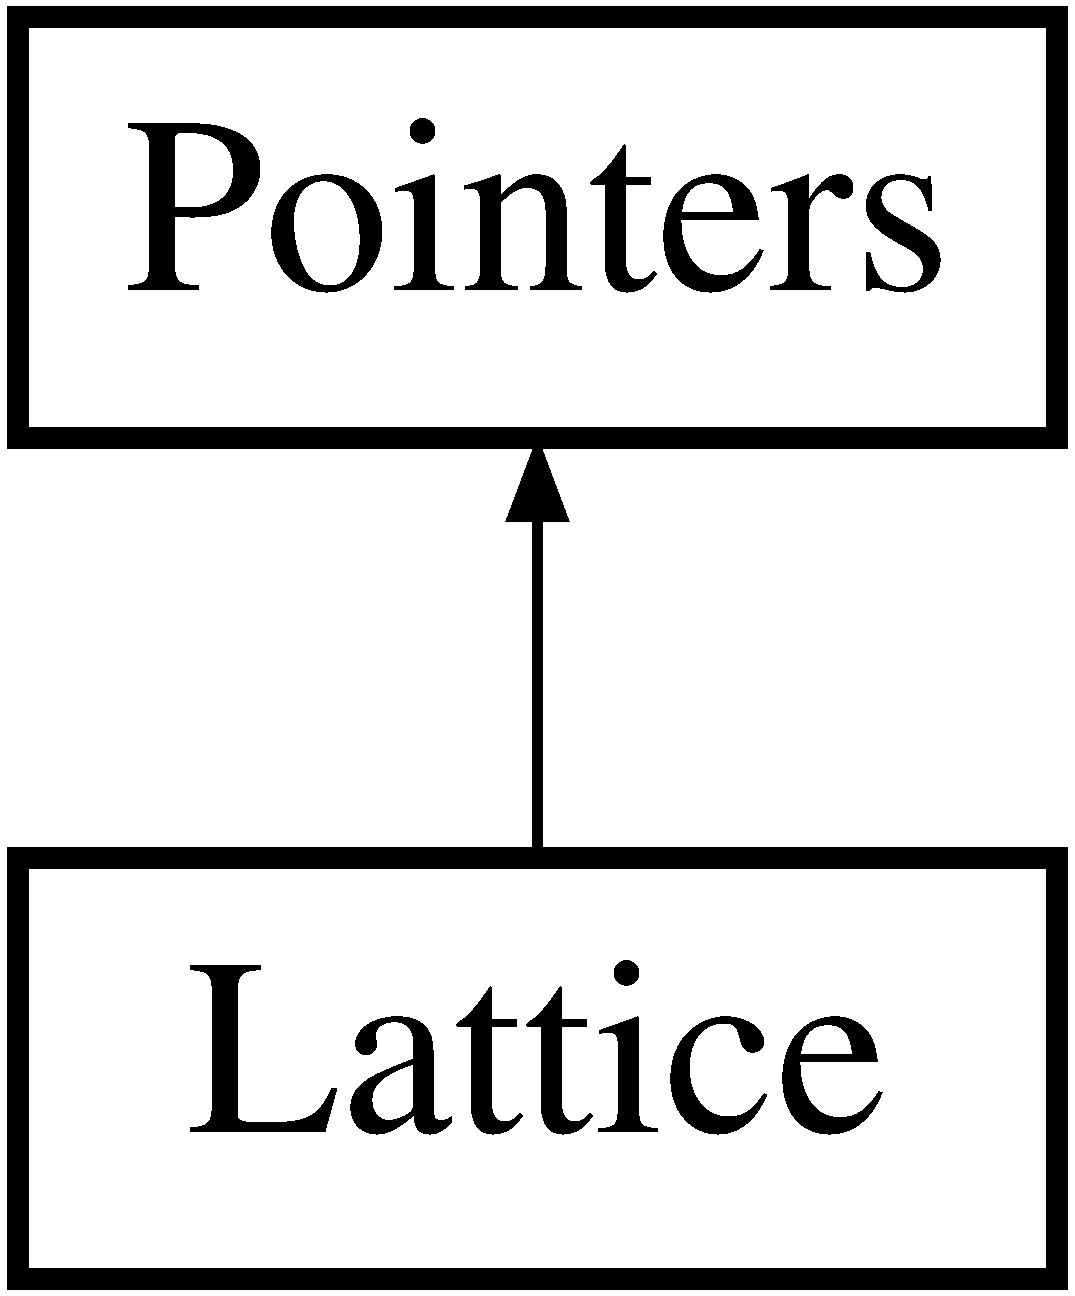
\includegraphics[height=2.000000cm]{classLattice}
\end{center}
\end{figure}
\subsection*{Public Types}
\begin{DoxyCompactItemize}
\item 
\mbox{\Hypertarget{classLattice_a0521158021627f01f6bb0a9c72df65e2}\label{classLattice_a0521158021627f01f6bb0a9c72df65e2}} 
enum \mbox{\hyperlink{classLattice_a0521158021627f01f6bb0a9c72df65e2}{Type}} \{ {\bfseries N\+O\+NE}, 
{\bfseries B\+CC}, 
{\bfseries F\+CC}
 \}
\begin{DoxyCompactList}\small\item\em The type of the lattice. \end{DoxyCompactList}\end{DoxyCompactItemize}
\subsection*{Public Member Functions}
\begin{DoxyCompactItemize}
\item 
\mbox{\Hypertarget{classLattice_a2a692cb14beaf2833c7997ff1adbca97}\label{classLattice_a2a692cb14beaf2833c7997ff1adbca97}} 
\mbox{\hyperlink{classLattice_a2a692cb14beaf2833c7997ff1adbca97}{Lattice}} (\mbox{\hyperlink{classApothesis}{Apothesis}} $\ast$apothesis)
\begin{DoxyCompactList}\small\item\em Constructor. \end{DoxyCompactList}\item 
\mbox{\Hypertarget{classLattice_a91be54ce9927b6bc53d30a2faf760780}\label{classLattice_a91be54ce9927b6bc53d30a2faf760780}} 
virtual \mbox{\hyperlink{classLattice_a91be54ce9927b6bc53d30a2faf760780}{$\sim$\+Lattice}} ()
\begin{DoxyCompactList}\small\item\em Distructor. \end{DoxyCompactList}\item 
\mbox{\Hypertarget{classLattice_a89814b38f15333f57e88ce4321f0796f}\label{classLattice_a89814b38f15333f57e88ce4321f0796f}} 
void \mbox{\hyperlink{classLattice_a89814b38f15333f57e88ce4321f0796f}{set\+Type}} (string)
\begin{DoxyCompactList}\small\item\em Sets the type of the lattice. \end{DoxyCompactList}\item 
\mbox{\Hypertarget{classLattice_a089ba222dac9bfac95cc4142d9886a9b}\label{classLattice_a089ba222dac9bfac95cc4142d9886a9b}} 
int \mbox{\hyperlink{classLattice_a089ba222dac9bfac95cc4142d9886a9b}{getX}} ()
\begin{DoxyCompactList}\small\item\em Returns the x dimension of the lattice. \end{DoxyCompactList}\item 
\mbox{\Hypertarget{classLattice_ae49e9c8208141bd28c2dcf12b93f3db1}\label{classLattice_ae49e9c8208141bd28c2dcf12b93f3db1}} 
int \mbox{\hyperlink{classLattice_ae49e9c8208141bd28c2dcf12b93f3db1}{getY}} ()
\begin{DoxyCompactList}\small\item\em Returns the y dimension of the lattice. \end{DoxyCompactList}\item 
\mbox{\Hypertarget{classLattice_ae134aa0d64a69678c9c6f00b7a9e7945}\label{classLattice_ae134aa0d64a69678c9c6f00b7a9e7945}} 
int \mbox{\hyperlink{classLattice_ae134aa0d64a69678c9c6f00b7a9e7945}{get\+Size}} ()
\begin{DoxyCompactList}\small\item\em Returns the size of the lattice. \end{DoxyCompactList}\item 
\mbox{\Hypertarget{classLattice_a7d24123500b25d2bc7e024827f5b3be4}\label{classLattice_a7d24123500b25d2bc7e024827f5b3be4}} 
\mbox{\hyperlink{classLattice_a0521158021627f01f6bb0a9c72df65e2}{Lattice\+::\+Type}} \mbox{\hyperlink{classLattice_a7d24123500b25d2bc7e024827f5b3be4}{get\+Type}} ()
\begin{DoxyCompactList}\small\item\em Returns the type of the lattice. \end{DoxyCompactList}\item 
\mbox{\Hypertarget{classLattice_aceabd17451b9dbb6dc6836f0bc007a29}\label{classLattice_aceabd17451b9dbb6dc6836f0bc007a29}} 
\mbox{\hyperlink{classSurfaceTiles_1_1Site}{Site}} $\ast$ \mbox{\hyperlink{classLattice_aceabd17451b9dbb6dc6836f0bc007a29}{get\+Lattice}} ()
\begin{DoxyCompactList}\small\item\em Returns the lattice. \end{DoxyCompactList}\item 
\mbox{\Hypertarget{classLattice_a3fc011bc7d8f6bdf230c64dff0d1ede5}\label{classLattice_a3fc011bc7d8f6bdf230c64dff0d1ede5}} 
\mbox{\hyperlink{classSurfaceTiles_1_1Site}{Site}} $\ast$ \mbox{\hyperlink{classLattice_a3fc011bc7d8f6bdf230c64dff0d1ede5}{get\+Site}} (int id)
\begin{DoxyCompactList}\small\item\em Returns a site with a specific id. \end{DoxyCompactList}\item 
\mbox{\Hypertarget{classLattice_a2e04013b9daf15281f1c21aafe0c3964}\label{classLattice_a2e04013b9daf15281f1c21aafe0c3964}} 
vector$<$ \mbox{\hyperlink{classSurfaceTiles_1_1Site}{Site}} $\ast$ $>$ \mbox{\hyperlink{classLattice_a2e04013b9daf15281f1c21aafe0c3964}{get\+Sites}} ()
\begin{DoxyCompactList}\small\item\em Returns all the sites of the lattice. \end{DoxyCompactList}\item 
\mbox{\Hypertarget{classLattice_ad85ed4a582942c2ae7346f3e3177e962}\label{classLattice_ad85ed4a582942c2ae7346f3e3177e962}} 
void \mbox{\hyperlink{classLattice_ad85ed4a582942c2ae7346f3e3177e962}{check}} ()
\begin{DoxyCompactList}\small\item\em Various checks if the lattice has been constucted correctly. Partially implemented. \end{DoxyCompactList}\item 
\mbox{\Hypertarget{classLattice_af4b8aea57fbe61b8c99352a56b88ecdd}\label{classLattice_af4b8aea57fbe61b8c99352a56b88ecdd}} 
void \mbox{\hyperlink{classLattice_af4b8aea57fbe61b8c99352a56b88ecdd}{init}} ()
\begin{DoxyCompactList}\small\item\em Init the lattice. \end{DoxyCompactList}\item 
\mbox{\Hypertarget{classLattice_a0bfe2ce023eded6bac20ba652b93eab2}\label{classLattice_a0bfe2ce023eded6bac20ba652b93eab2}} 
void \mbox{\hyperlink{classLattice_a0bfe2ce023eded6bac20ba652b93eab2}{set\+Type}} (\mbox{\hyperlink{classLattice_a0521158021627f01f6bb0a9c72df65e2}{Type}} type)
\begin{DoxyCompactList}\small\item\em Set the type of the lattice. \end{DoxyCompactList}\item 
\mbox{\Hypertarget{classLattice_a195be05258d896fe3342e4eac2f3ffee}\label{classLattice_a195be05258d896fe3342e4eac2f3ffee}} 
void \mbox{\hyperlink{classLattice_a195be05258d896fe3342e4eac2f3ffee}{setX}} (int x)
\begin{DoxyCompactList}\small\item\em Set the X dimension of the lattice. \end{DoxyCompactList}\item 
\mbox{\Hypertarget{classLattice_ae79cea22c63903e846d4858250b80ed9}\label{classLattice_ae79cea22c63903e846d4858250b80ed9}} 
void \mbox{\hyperlink{classLattice_ae79cea22c63903e846d4858250b80ed9}{setY}} (int y)
\begin{DoxyCompactList}\small\item\em Set the Y dimension of the lattice. \end{DoxyCompactList}\item 
\mbox{\Hypertarget{classLattice_a079f2eedf2fcdd34a85766a4f08ca9c4}\label{classLattice_a079f2eedf2fcdd34a85766a4f08ca9c4}} 
void \mbox{\hyperlink{classLattice_a079f2eedf2fcdd34a85766a4f08ca9c4}{build}} ()
\begin{DoxyCompactList}\small\item\em Build the lattice with an intitial height. \end{DoxyCompactList}\item 
\mbox{\Hypertarget{classLattice_a3d953999db7b36864a89aea221a1ddc6}\label{classLattice_a3d953999db7b36864a89aea221a1ddc6}} 
void \mbox{\hyperlink{classLattice_a3d953999db7b36864a89aea221a1ddc6}{set\+Initial\+Height}} (int height)
\begin{DoxyCompactList}\small\item\em Sets the minimun initial height for the lattice. \end{DoxyCompactList}\end{DoxyCompactItemize}
\subsection*{Protected Member Functions}
\begin{DoxyCompactItemize}
\item 
\mbox{\Hypertarget{classLattice_a0f932c1ad96eaaa2dcee0cec3da16c2a}\label{classLattice_a0f932c1ad96eaaa2dcee0cec3da16c2a}} 
void \mbox{\hyperlink{classLattice_a0f932c1ad96eaaa2dcee0cec3da16c2a}{mf\+\_\+fcc\+Neigh}} ()
\begin{DoxyCompactList}\small\item\em The neighbours for the F\+CC lattice. \end{DoxyCompactList}\item 
\mbox{\Hypertarget{classLattice_a70f6567232ec6739b19afecb5ef7f79c}\label{classLattice_a70f6567232ec6739b19afecb5ef7f79c}} 
void \mbox{\hyperlink{classLattice_a70f6567232ec6739b19afecb5ef7f79c}{mf\+\_\+build\+Neighbours}} ()
\begin{DoxyCompactList}\small\item\em Build the neighbours of each site depending on the type of the. \end{DoxyCompactList}\end{DoxyCompactItemize}
\subsection*{Protected Attributes}
\begin{DoxyCompactItemize}
\item 
\mbox{\Hypertarget{classLattice_ad965735fabbea7f2cd4fd841e3905714}\label{classLattice_ad965735fabbea7f2cd4fd841e3905714}} 
int \mbox{\hyperlink{classLattice_ad965735fabbea7f2cd4fd841e3905714}{m\+\_\+i\+SizeX}}
\begin{DoxyCompactList}\small\item\em The size of the lattice in the x-\/dimension. \end{DoxyCompactList}\item 
\mbox{\Hypertarget{classLattice_a9c396b8ce6a9b4401a7f1f174e1a743d}\label{classLattice_a9c396b8ce6a9b4401a7f1f174e1a743d}} 
int \mbox{\hyperlink{classLattice_a9c396b8ce6a9b4401a7f1f174e1a743d}{m\+\_\+i\+SizeY}}
\begin{DoxyCompactList}\small\item\em The size of the lattice in the y-\/dimension. \end{DoxyCompactList}\item 
\mbox{\Hypertarget{classLattice_a41e09891128085d8d324c11267f27ef5}\label{classLattice_a41e09891128085d8d324c11267f27ef5}} 
int \mbox{\hyperlink{classLattice_a41e09891128085d8d324c11267f27ef5}{m\+\_\+i\+Height}}
\begin{DoxyCompactList}\small\item\em The minimum initialize size of the lattice. \end{DoxyCompactList}\item 
\mbox{\Hypertarget{classLattice_a81dd6a7c57c02a8172544d7b67b84a16}\label{classLattice_a81dd6a7c57c02a8172544d7b67b84a16}} 
\mbox{\hyperlink{classLattice_a0521158021627f01f6bb0a9c72df65e2}{Type}} \mbox{\hyperlink{classLattice_a81dd6a7c57c02a8172544d7b67b84a16}{m\+\_\+\+Type}}
\begin{DoxyCompactList}\small\item\em The type of the lattice\+: B\+CC, F\+CC etc. \end{DoxyCompactList}\item 
\mbox{\Hypertarget{classLattice_abefaff3c5de9ff49cc0e61d4a8259c93}\label{classLattice_abefaff3c5de9ff49cc0e61d4a8259c93}} 
vector$<$ \mbox{\hyperlink{classSurfaceTiles_1_1Site}{Site}} $\ast$$>$ \mbox{\hyperlink{classLattice_abefaff3c5de9ff49cc0e61d4a8259c93}{m\+\_\+v\+Sites}}
\begin{DoxyCompactList}\small\item\em The sites that consist the lattice. \end{DoxyCompactList}\end{DoxyCompactItemize}


The documentation for this class was generated from the following files\+:\begin{DoxyCompactItemize}
\item 
lattice.\+h\item 
lattice.\+cpp\end{DoxyCompactItemize}

\hypertarget{classUtils_1_1Parameters}{}\section{Utils\+:\+:Parameters Class Reference}
\label{classUtils_1_1Parameters}\index{Utils\+::\+Parameters@{Utils\+::\+Parameters}}


{\ttfamily \#include $<$parameters.\+h$>$}

Inheritance diagram for Utils\+:\+:Parameters\+:\begin{figure}[H]
\begin{center}
\leavevmode
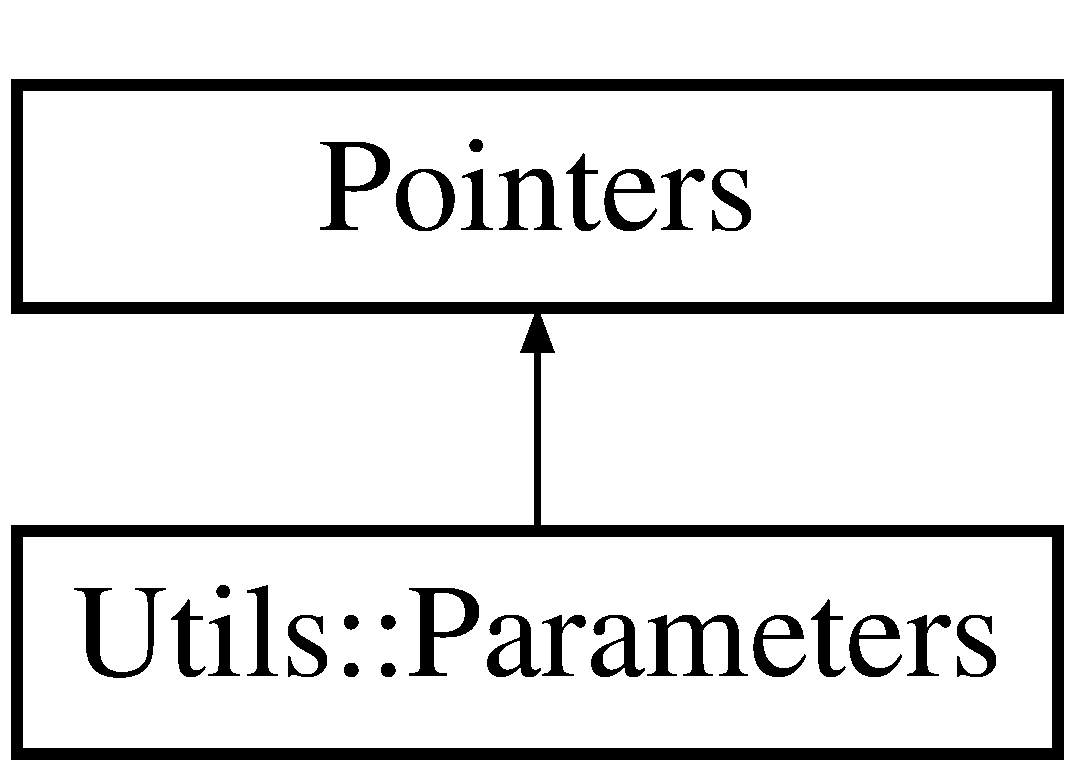
\includegraphics[height=2.000000cm]{classUtils_1_1Parameters}
\end{center}
\end{figure}
\subsection*{Public Member Functions}
\begin{DoxyCompactItemize}
\item 
\mbox{\Hypertarget{classUtils_1_1Parameters_a380d08553bc406d2cc3e2e4885a68de2}\label{classUtils_1_1Parameters_a380d08553bc406d2cc3e2e4885a68de2}} 
\mbox{\hyperlink{classUtils_1_1Parameters_a380d08553bc406d2cc3e2e4885a68de2}{Parameters}} (\mbox{\hyperlink{classApothesis}{Apothesis}} $\ast$apothesis)
\begin{DoxyCompactList}\small\item\em Constructor. \end{DoxyCompactList}\item 
\mbox{\Hypertarget{classUtils_1_1Parameters_a3e7985fcdc6cc28fdd178c503ab4a71f}\label{classUtils_1_1Parameters_a3e7985fcdc6cc28fdd178c503ab4a71f}} 
\mbox{\hyperlink{classUtils_1_1Parameters_a3e7985fcdc6cc28fdd178c503ab4a71f}{$\sim$\+Parameters}} ()
\begin{DoxyCompactList}\small\item\em Destructor. \end{DoxyCompactList}\item 
\mbox{\Hypertarget{classUtils_1_1Parameters_a2c4ca8ee4caffed82b37de23b04f27a3}\label{classUtils_1_1Parameters_a2c4ca8ee4caffed82b37de23b04f27a3}} 
void \mbox{\hyperlink{classUtils_1_1Parameters_a2c4ca8ee4caffed82b37de23b04f27a3}{set\+Temperature}} (double T)
\begin{DoxyCompactList}\small\item\em Set the temperature value. \end{DoxyCompactList}\item 
\mbox{\Hypertarget{classUtils_1_1Parameters_abb85d8b05fbe6d29673fc38af858f57c}\label{classUtils_1_1Parameters_abb85d8b05fbe6d29673fc38af858f57c}} 
double \mbox{\hyperlink{classUtils_1_1Parameters_abb85d8b05fbe6d29673fc38af858f57c}{get\+Temperature}} ()
\begin{DoxyCompactList}\small\item\em Get the temperature value. \end{DoxyCompactList}\item 
\mbox{\Hypertarget{classUtils_1_1Parameters_a7011b133a1474ea8ebcc05b16445a0cb}\label{classUtils_1_1Parameters_a7011b133a1474ea8ebcc05b16445a0cb}} 
void \mbox{\hyperlink{classUtils_1_1Parameters_a7011b133a1474ea8ebcc05b16445a0cb}{set\+Pressure}} (double)
\begin{DoxyCompactList}\small\item\em Set the pressure value. \end{DoxyCompactList}\item 
\mbox{\Hypertarget{classUtils_1_1Parameters_aa24d0f50720f02d44c6eccba5f2864ca}\label{classUtils_1_1Parameters_aa24d0f50720f02d44c6eccba5f2864ca}} 
double \mbox{\hyperlink{classUtils_1_1Parameters_aa24d0f50720f02d44c6eccba5f2864ca}{get\+Pressure}} ()
\begin{DoxyCompactList}\small\item\em Get the pressure value. \end{DoxyCompactList}\item 
\mbox{\Hypertarget{classUtils_1_1Parameters_a68dfe891b7f1a26d7bafa8cbc8488a22}\label{classUtils_1_1Parameters_a68dfe891b7f1a26d7bafa8cbc8488a22}} 
void \mbox{\hyperlink{classUtils_1_1Parameters_a68dfe891b7f1a26d7bafa8cbc8488a22}{set\+Iterations}} (int iter)
\begin{DoxyCompactList}\small\item\em Set the total number of K\+MC iterations. \end{DoxyCompactList}\item 
\mbox{\Hypertarget{classUtils_1_1Parameters_a164509763c6ddbcc095aa7ab24bb4491}\label{classUtils_1_1Parameters_a164509763c6ddbcc095aa7ab24bb4491}} 
int \mbox{\hyperlink{classUtils_1_1Parameters_a164509763c6ddbcc095aa7ab24bb4491}{get\+Iterations}} ()
\begin{DoxyCompactList}\small\item\em Set the total number of K\+MC iterations. \end{DoxyCompactList}\item 
\mbox{\Hypertarget{classUtils_1_1Parameters_ac51d57f8c27ad1d50d9f0c08b714ac6f}\label{classUtils_1_1Parameters_ac51d57f8c27ad1d50d9f0c08b714ac6f}} 
void \mbox{\hyperlink{classUtils_1_1Parameters_ac51d57f8c27ad1d50d9f0c08b714ac6f}{set\+Process}} (string, vector$<$ double $>$)
\begin{DoxyCompactList}\small\item\em Store the processes to be created by the factory method. \end{DoxyCompactList}\item 
\mbox{\Hypertarget{classUtils_1_1Parameters_a2ae018731d1166e2ecbb290946280979}\label{classUtils_1_1Parameters_a2ae018731d1166e2ecbb290946280979}} 
map$<$ string, vector$<$ double $>$ $>$ \mbox{\hyperlink{classUtils_1_1Parameters_a2ae018731d1166e2ecbb290946280979}{get\+Processes}} ()
\begin{DoxyCompactList}\small\item\em Get the processes to be created. \end{DoxyCompactList}\end{DoxyCompactItemize}
\subsection*{Public Attributes}
\begin{DoxyCompactItemize}
\item 
\mbox{\Hypertarget{classUtils_1_1Parameters_adce7e8fb0230d27d1553c05d793bcf97}\label{classUtils_1_1Parameters_adce7e8fb0230d27d1553c05d793bcf97}} 
const double \mbox{\hyperlink{classUtils_1_1Parameters_adce7e8fb0230d27d1553c05d793bcf97}{d\+Avogadro\+Num}} = 6.\+022141793e+23
\begin{DoxyCompactList}\small\item\em The Avogadro number. \end{DoxyCompactList}\item 
\mbox{\Hypertarget{classUtils_1_1Parameters_ab812c09a17b16a614115b80995aac582}\label{classUtils_1_1Parameters_ab812c09a17b16a614115b80995aac582}} 
const double \mbox{\hyperlink{classUtils_1_1Parameters_ab812c09a17b16a614115b80995aac582}{dk\+Boltz}} = 1.\+3806503e-\/23
\begin{DoxyCompactList}\small\item\em The boltzmann constant. \end{DoxyCompactList}\item 
\mbox{\Hypertarget{classUtils_1_1Parameters_a7118286f5e28f6eb7944d7c04e729e32}\label{classUtils_1_1Parameters_a7118286f5e28f6eb7944d7c04e729e32}} 
const double \mbox{\hyperlink{classUtils_1_1Parameters_a7118286f5e28f6eb7944d7c04e729e32}{d\+Pi}} = 3.\+14159265
\begin{DoxyCompactList}\small\item\em Pi. \end{DoxyCompactList}\end{DoxyCompactItemize}
\subsection*{Protected Attributes}
\begin{DoxyCompactItemize}
\item 
\mbox{\Hypertarget{classUtils_1_1Parameters_ae876725df0b9ced07288603b77014fc5}\label{classUtils_1_1Parameters_ae876725df0b9ced07288603b77014fc5}} 
double \mbox{\hyperlink{classUtils_1_1Parameters_ae876725df0b9ced07288603b77014fc5}{m\+\_\+dT}}
\begin{DoxyCompactList}\small\item\em The temperature. \end{DoxyCompactList}\item 
\mbox{\Hypertarget{classUtils_1_1Parameters_a464c3be85185b6eae1397e9dab04d295}\label{classUtils_1_1Parameters_a464c3be85185b6eae1397e9dab04d295}} 
double \mbox{\hyperlink{classUtils_1_1Parameters_a464c3be85185b6eae1397e9dab04d295}{m\+\_\+dP}}
\begin{DoxyCompactList}\small\item\em The pressure. \end{DoxyCompactList}\item 
\mbox{\Hypertarget{classUtils_1_1Parameters_a93a7064eaaa706a00ad584ccd6a984ba}\label{classUtils_1_1Parameters_a93a7064eaaa706a00ad584ccd6a984ba}} 
int \mbox{\hyperlink{classUtils_1_1Parameters_a93a7064eaaa706a00ad584ccd6a984ba}{m\+\_\+i\+Iter}}
\begin{DoxyCompactList}\small\item\em The number of iterations to be performed. \end{DoxyCompactList}\item 
\mbox{\Hypertarget{classUtils_1_1Parameters_af280da145e43025392232ac12351a0f6}\label{classUtils_1_1Parameters_af280da145e43025392232ac12351a0f6}} 
map$<$ string, vector$<$ double $>$ $>$ \mbox{\hyperlink{classUtils_1_1Parameters_af280da145e43025392232ac12351a0f6}{m\+\_\+m\+Procs}}
\begin{DoxyCompactList}\small\item\em Stores the processes as read from the input file allong with their parameters. \end{DoxyCompactList}\end{DoxyCompactItemize}


\subsection{Detailed Description}
A class which hold all the parameters needed by K\+MC. Other parameters needed by the individual processes can be defined there. 

The documentation for this class was generated from the following files\+:\begin{DoxyCompactItemize}
\item 
parameters.\+h\item 
parameters.\+cpp\end{DoxyCompactItemize}

\hypertarget{classPointers}{}\section{Pointers Class Reference}
\label{classPointers}\index{Pointers@{Pointers}}


{\ttfamily \#include $<$pointers.\+h$>$}

Inheritance diagram for Pointers\+:\begin{figure}[H]
\begin{center}
\leavevmode
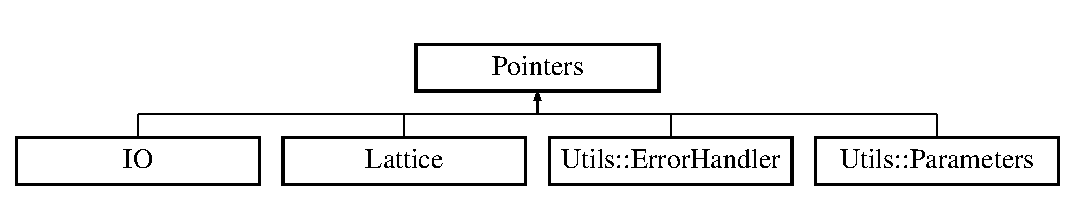
\includegraphics[height=2.000000cm]{classPointers}
\end{center}
\end{figure}
\subsection*{Public Member Functions}
\begin{DoxyCompactItemize}
\item 
\mbox{\Hypertarget{classPointers_affc1e7aa2bea5b24f4b03660d64897da}\label{classPointers_affc1e7aa2bea5b24f4b03660d64897da}} 
\mbox{\hyperlink{classPointers_affc1e7aa2bea5b24f4b03660d64897da}{Pointers}} (\mbox{\hyperlink{classApothesis}{Apothesis}} $\ast$apothesis)
\begin{DoxyCompactList}\small\item\em Contructor. \end{DoxyCompactList}\end{DoxyCompactItemize}
\subsection*{Protected Attributes}
\begin{DoxyCompactItemize}
\item 
\mbox{\Hypertarget{classPointers_a2573d2d29e2ee82e5eb351e9b340297f}\label{classPointers_a2573d2d29e2ee82e5eb351e9b340297f}} 
\mbox{\hyperlink{classApothesis}{Apothesis}} $\ast$\& \mbox{\hyperlink{classPointers_a2573d2d29e2ee82e5eb351e9b340297f}{m\+\_\+apothesis}}
\begin{DoxyCompactList}\small\item\em \mbox{\hyperlink{classPointers}{Pointers}} to the classes of kmc.\+cpp. \end{DoxyCompactList}\item 
\mbox{\Hypertarget{classPointers_aed3e1462a45bffbe51b2de8fb36ea5a0}\label{classPointers_aed3e1462a45bffbe51b2de8fb36ea5a0}} 
\mbox{\hyperlink{classLattice}{Lattice}} $\ast$\& \mbox{\hyperlink{classPointers_aed3e1462a45bffbe51b2de8fb36ea5a0}{m\+\_\+lattice}}
\begin{DoxyCompactList}\small\item\em \mbox{\hyperlink{classPointers}{Pointers}} to the classes of kmc.\+cpp. \end{DoxyCompactList}\item 
\mbox{\Hypertarget{classPointers_aff865007d21415a6ee4a8b03ad3c1bc5}\label{classPointers_aff865007d21415a6ee4a8b03ad3c1bc5}} 
\mbox{\hyperlink{classIO}{IO}} $\ast$\& \mbox{\hyperlink{classPointers_aff865007d21415a6ee4a8b03ad3c1bc5}{m\+\_\+io}}
\begin{DoxyCompactList}\small\item\em \mbox{\hyperlink{classPointers}{Pointers}} to the classes of kmc.\+cpp. \end{DoxyCompactList}\item 
\mbox{\Hypertarget{classPointers_a38807af78210f98930ae491abb9ebf68}\label{classPointers_a38807af78210f98930ae491abb9ebf68}} 
\mbox{\hyperlink{classUtils_1_1ErrorHandler}{Utils\+::\+Error\+Handler}} $\ast$\& \mbox{\hyperlink{classPointers_a38807af78210f98930ae491abb9ebf68}{m\+\_\+error\+Handler}}
\begin{DoxyCompactList}\small\item\em \mbox{\hyperlink{classPointers}{Pointers}} to the classes of kmc.\+cpp. \end{DoxyCompactList}\item 
\mbox{\Hypertarget{classPointers_ac0cc2a98afeec07800eca1828978e322}\label{classPointers_ac0cc2a98afeec07800eca1828978e322}} 
\mbox{\hyperlink{classUtils_1_1Parameters}{Utils\+::\+Parameters}} $\ast$\& \mbox{\hyperlink{classPointers_ac0cc2a98afeec07800eca1828978e322}{m\+\_\+parameters}}
\begin{DoxyCompactList}\small\item\em \mbox{\hyperlink{classPointers}{Pointers}} to the classes of kmc.\+cpp. \end{DoxyCompactList}\end{DoxyCompactItemize}


\subsection{Detailed Description}
The pointers class contains pointers to the classes defined in kmc.\+cpp. Itcreates a common space of all the class instances that are defined in the kmc class. As long as a kmc instance exists these classes are \char`\"{}united\char`\"{} in this common space. So, if someone wants to use the lattice instance from the io instance all that has to do is to call the insance as this defined in the kmc.\+cpp. For example in kcc.\+cpp an instance of the class lattice is p\+Lattice and an object of the io class is p\+IO. If someones wants to use the p\+IO from p\+Lattice all (s)he has to do is to call p\+I\+O-\/$>$ and the relevant public functionalities of the class. This is very handy to bind together different instances. (Taken from L\+A\+M\+M\+PS ;) ) 

The documentation for this class was generated from the following file\+:\begin{DoxyCompactItemize}
\item 
pointers.\+h\end{DoxyCompactItemize}

\hypertarget{classMicroProcesses_1_1Process}{}\section{Micro\+Processes\+:\+:Process Class Reference}
\label{classMicroProcesses_1_1Process}\index{Micro\+Processes\+::\+Process@{Micro\+Processes\+::\+Process}}
Inheritance diagram for Micro\+Processes\+:\+:Process\+:\begin{figure}[H]
\begin{center}
\leavevmode
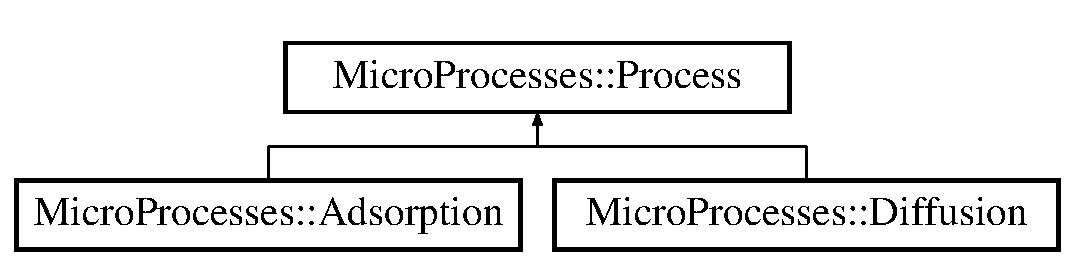
\includegraphics[height=2.000000cm]{classMicroProcesses_1_1Process}
\end{center}
\end{figure}
\subsection*{Public Member Functions}
\begin{DoxyCompactItemize}
\item 
\mbox{\Hypertarget{classMicroProcesses_1_1Process_ac0ed6a31edbe810d849cff9ab6da1233}\label{classMicroProcesses_1_1Process_ac0ed6a31edbe810d849cff9ab6da1233}} 
\mbox{\hyperlink{classMicroProcesses_1_1Process_ac0ed6a31edbe810d849cff9ab6da1233}{Process}} ()
\begin{DoxyCompactList}\small\item\em Constructor of the interface. \end{DoxyCompactList}\item 
\mbox{\Hypertarget{classMicroProcesses_1_1Process_a093d6dc68f2e95ad6129623996853863}\label{classMicroProcesses_1_1Process_a093d6dc68f2e95ad6129623996853863}} 
virtual \mbox{\hyperlink{classMicroProcesses_1_1Process_a093d6dc68f2e95ad6129623996853863}{$\sim$\+Process}} ()
\begin{DoxyCompactList}\small\item\em Destructor. \end{DoxyCompactList}\item 
\mbox{\Hypertarget{classMicroProcesses_1_1Process_a54c59b0eb502785edd0df976e232aeb1}\label{classMicroProcesses_1_1Process_a54c59b0eb502785edd0df976e232aeb1}} 
virtual void \mbox{\hyperlink{classMicroProcesses_1_1Process_a54c59b0eb502785edd0df976e232aeb1}{set\+Name}} (string s)=0
\begin{DoxyCompactList}\small\item\em Set the name of the process. \end{DoxyCompactList}\item 
\mbox{\Hypertarget{classMicroProcesses_1_1Process_a1933fe53e2545c533ab9de6a094437f9}\label{classMicroProcesses_1_1Process_a1933fe53e2545c533ab9de6a094437f9}} 
virtual string \mbox{\hyperlink{classMicroProcesses_1_1Process_a1933fe53e2545c533ab9de6a094437f9}{get\+Name}} ()=0
\begin{DoxyCompactList}\small\item\em Get the name of the process. \end{DoxyCompactList}\item 
\mbox{\Hypertarget{classMicroProcesses_1_1Process_ae6414c8655f64aa691912db2aec8ad17}\label{classMicroProcesses_1_1Process_ae6414c8655f64aa691912db2aec8ad17}} 
virtual void \mbox{\hyperlink{classMicroProcesses_1_1Process_ae6414c8655f64aa691912db2aec8ad17}{active\+Sites}} (\mbox{\hyperlink{classLattice}{Lattice}} $\ast$)=0
\begin{DoxyCompactList}\small\item\em Constructs the sites that a process can be performed. \end{DoxyCompactList}\item 
virtual void \mbox{\hyperlink{classMicroProcesses_1_1Process_a5b0a36197e03be4f36465a6b9d4f867f}{select\+Site}} ()=0
\item 
\mbox{\Hypertarget{classMicroProcesses_1_1Process_a4e726f7491eb805efd9dcd1c0c3a380f}\label{classMicroProcesses_1_1Process_a4e726f7491eb805efd9dcd1c0c3a380f}} 
virtual void \mbox{\hyperlink{classMicroProcesses_1_1Process_a4e726f7491eb805efd9dcd1c0c3a380f}{set\+Process\+Map}} (map$<$ \mbox{\hyperlink{classMicroProcesses_1_1Process}{Process}} $\ast$, list$<$ \mbox{\hyperlink{classSurfaceTiles_1_1Site}{Site}} $\ast$ $>$ $\ast$ $>$ $\ast$)=0
\begin{DoxyCompactList}\small\item\em The process map which holds all the processes and the sites that each can be performed. \end{DoxyCompactList}\item 
\mbox{\Hypertarget{classMicroProcesses_1_1Process_a4247eaf16a8ea1f9b4df0d99efe3287e}\label{classMicroProcesses_1_1Process_a4247eaf16a8ea1f9b4df0d99efe3287e}} 
virtual void \mbox{\hyperlink{classMicroProcesses_1_1Process_a4247eaf16a8ea1f9b4df0d99efe3287e}{perform}} ()=0
\begin{DoxyCompactList}\small\item\em Perform the process. \end{DoxyCompactList}\item 
\mbox{\Hypertarget{classMicroProcesses_1_1Process_a76c7fededf36c867251c6b803f7841bf}\label{classMicroProcesses_1_1Process_a76c7fededf36c867251c6b803f7841bf}} 
virtual double \mbox{\hyperlink{classMicroProcesses_1_1Process_a76c7fededf36c867251c6b803f7841bf}{get\+Probability}} ()=0
\begin{DoxyCompactList}\small\item\em Calculate and get the Probability of this process. \end{DoxyCompactList}\item 
virtual list$<$ \mbox{\hyperlink{classSurfaceTiles_1_1Site}{Site}} $\ast$$>$ \mbox{\hyperlink{classMicroProcesses_1_1Process_ab2b962d50cca475005fd6d6477258e58}{get\+Active\+List}} ()=0
\item 
\mbox{\Hypertarget{classMicroProcesses_1_1Process_a4c419af2e6e6477200b45bf687783c84}\label{classMicroProcesses_1_1Process_a4c419af2e6e6477200b45bf687783c84}} 
virtual void \mbox{\hyperlink{classMicroProcesses_1_1Process_a4c419af2e6e6477200b45bf687783c84}{set\+Instance}} (\mbox{\hyperlink{classApothesis}{Apothesis}} $\ast$apothesis)=0
\begin{DoxyCompactList}\small\item\em Set the instance of kmc that this process will be performed. \end{DoxyCompactList}\end{DoxyCompactItemize}


\subsection{Member Function Documentation}
\mbox{\Hypertarget{classMicroProcesses_1_1Process_ab2b962d50cca475005fd6d6477258e58}\label{classMicroProcesses_1_1Process_ab2b962d50cca475005fd6d6477258e58}} 
\index{Micro\+Processes\+::\+Process@{Micro\+Processes\+::\+Process}!get\+Active\+List@{get\+Active\+List}}
\index{get\+Active\+List@{get\+Active\+List}!Micro\+Processes\+::\+Process@{Micro\+Processes\+::\+Process}}
\subsubsection{\texorpdfstring{get\+Active\+List()}{getActiveList()}}
{\footnotesize\ttfamily virtual list$<$\mbox{\hyperlink{classSurfaceTiles_1_1Site}{Site}}$\ast$ $>$ Micro\+Processes\+::\+Process\+::get\+Active\+List (\begin{DoxyParamCaption}{ }\end{DoxyParamCaption})\hspace{0.3cm}{\ttfamily [pure virtual]}}

Get the list of active sites where the process can be performed. This is updated after a process is performed. 

Implemented in \mbox{\hyperlink{classMicroProcesses_1_1Adsorption_ac8bab3e2a04a6ea204c8f31077fb83fb}{Micro\+Processes\+::\+Adsorption}}, and \mbox{\hyperlink{classMicroProcesses_1_1Diffusion_a8e19130f8f9948f1a6a446f4065027dd}{Micro\+Processes\+::\+Diffusion}}.

\mbox{\Hypertarget{classMicroProcesses_1_1Process_a5b0a36197e03be4f36465a6b9d4f867f}\label{classMicroProcesses_1_1Process_a5b0a36197e03be4f36465a6b9d4f867f}} 
\index{Micro\+Processes\+::\+Process@{Micro\+Processes\+::\+Process}!select\+Site@{select\+Site}}
\index{select\+Site@{select\+Site}!Micro\+Processes\+::\+Process@{Micro\+Processes\+::\+Process}}
\subsubsection{\texorpdfstring{select\+Site()}{selectSite()}}
{\footnotesize\ttfamily virtual void Micro\+Processes\+::\+Process\+::select\+Site (\begin{DoxyParamCaption}{ }\end{DoxyParamCaption})\hspace{0.3cm}{\ttfamily [pure virtual]}}

The site that this process will be performed. The site is selected from the available sites that have been constructed in active\+Sites 

Implemented in \mbox{\hyperlink{classMicroProcesses_1_1Adsorption_af20402b5bfbc7b627ad8de13bdc2c541}{Micro\+Processes\+::\+Adsorption}}, and \mbox{\hyperlink{classMicroProcesses_1_1Diffusion_af699c30b1c182cce03e9a9826b0c5b51}{Micro\+Processes\+::\+Diffusion}}.



The documentation for this class was generated from the following file\+:\begin{DoxyCompactItemize}
\item 
process.\+h\end{DoxyCompactItemize}

\hypertarget{classRegister}{}\section{Register$<$ T $>$ Class Template Reference}
\label{classRegister}\index{Register$<$ T $>$@{Register$<$ T $>$}}


{\ttfamily \#include $<$register.\+h$>$}

Inheritance diagram for Register$<$ T $>$\+:\begin{figure}[H]
\begin{center}
\leavevmode
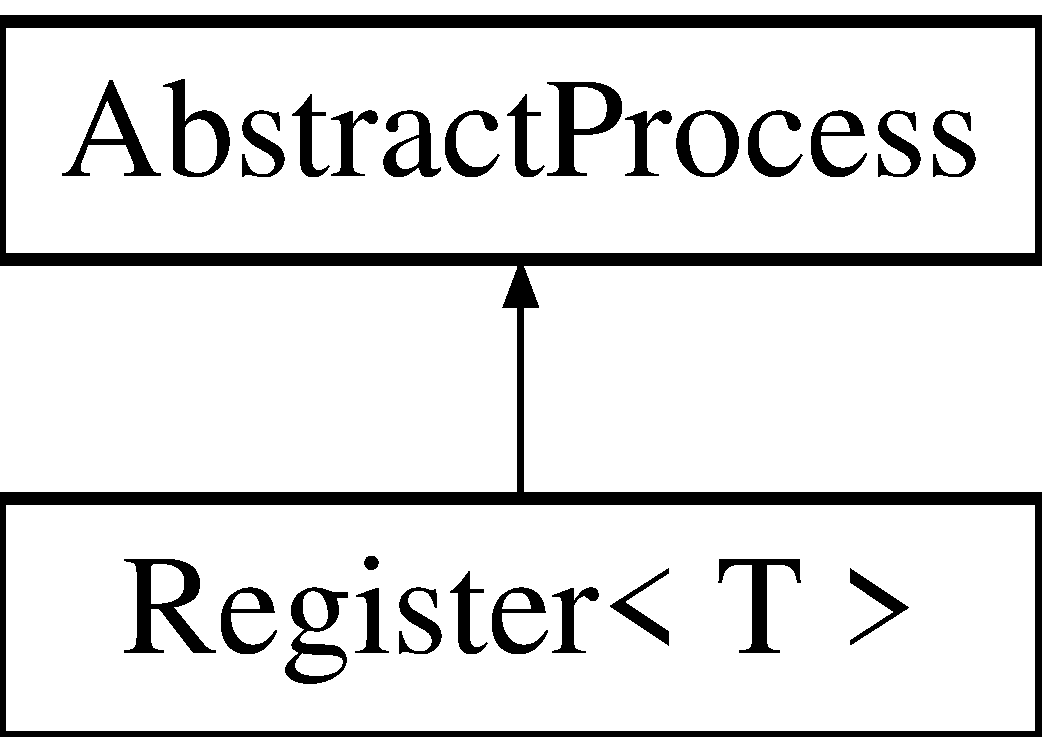
\includegraphics[height=2.000000cm]{classRegister}
\end{center}
\end{figure}
\subsection*{Public Member Functions}
\begin{DoxyCompactItemize}
\item 
\mbox{\Hypertarget{classRegister_a009b50170f81ae1cf3996fc713b13ab6}\label{classRegister_a009b50170f81ae1cf3996fc713b13ab6}} 
\mbox{\hyperlink{classRegister_a009b50170f81ae1cf3996fc713b13ab6}{Register}} (const std\+::string \&name)
\begin{DoxyCompactList}\small\item\em Contructor. \end{DoxyCompactList}\item 
\mbox{\Hypertarget{classRegister_a6ea38ad87b77e21ce8eaeb1aefd29cad}\label{classRegister_a6ea38ad87b77e21ce8eaeb1aefd29cad}} 
\mbox{\hyperlink{classRegister_a6ea38ad87b77e21ce8eaeb1aefd29cad}{$\sim$\+Register}} ()
\begin{DoxyCompactList}\small\item\em Destructor. \end{DoxyCompactList}\item 
\mbox{\Hypertarget{classRegister_abe8bb728066c0cdad90a6f631dc7a1d0}\label{classRegister_abe8bb728066c0cdad90a6f631dc7a1d0}} 
virtual \mbox{\hyperlink{classMicroProcesses_1_1Process}{Micro\+Processes\+::\+Process}} $\ast$ \mbox{\hyperlink{classRegister_abe8bb728066c0cdad90a6f631dc7a1d0}{create}} ()
\begin{DoxyCompactList}\small\item\em Creator of the process. \end{DoxyCompactList}\end{DoxyCompactItemize}


\subsection{Detailed Description}
\subsubsection*{template$<$class T$>$\newline
class Register$<$ T $>$}

A template class used by the factory method for creating the processes. 

The documentation for this class was generated from the following files\+:\begin{DoxyCompactItemize}
\item 
register.\+h\item 
register.\+cpp\end{DoxyCompactItemize}

\hypertarget{classSurfaceTiles_1_1Site}{}\section{Surface\+Tiles\+:\+:Site Class Reference}
\label{classSurfaceTiles_1_1Site}\index{Surface\+Tiles\+::\+Site@{Surface\+Tiles\+::\+Site}}
\subsection*{Public Types}
\begin{DoxyCompactItemize}
\item 
\mbox{\Hypertarget{classSurfaceTiles_1_1Site_a6cef4c767e7aa8320658fb3cd0fa3b1c}\label{classSurfaceTiles_1_1Site_a6cef4c767e7aa8320658fb3cd0fa3b1c}} 
enum \mbox{\hyperlink{classSurfaceTiles_1_1Site_a6cef4c767e7aa8320658fb3cd0fa3b1c}{Neigh\+Poisition}} \{ \newline
{\bfseries W\+E\+ST}, 
{\bfseries W\+E\+S\+T\+\_\+\+UP}, 
{\bfseries W\+E\+S\+T\+\_\+\+D\+O\+WN}, 
{\bfseries E\+A\+ST}, 
\newline
{\bfseries E\+A\+S\+T\+\_\+\+UP}, 
{\bfseries E\+A\+S\+T\+\_\+\+D\+O\+WN}, 
{\bfseries N\+O\+R\+TH}, 
{\bfseries S\+O\+U\+TH}
 \}
\begin{DoxyCompactList}\small\item\em The position of the neighbour. \end{DoxyCompactList}\item 
\mbox{\Hypertarget{classSurfaceTiles_1_1Site_a459d18c54ed5cbe4db365a2a0a4b6492}\label{classSurfaceTiles_1_1Site_a459d18c54ed5cbe4db365a2a0a4b6492}} 
enum \mbox{\hyperlink{classSurfaceTiles_1_1Site_a459d18c54ed5cbe4db365a2a0a4b6492}{Activation\+Site}} \{ \newline
{\bfseries A\+C\+T\+V\+\_\+\+W\+E\+ST}, 
{\bfseries A\+C\+T\+V\+\_\+\+W\+E\+S\+T\+\_\+\+UP}, 
{\bfseries A\+C\+T\+V\+\_\+\+W\+E\+S\+T\+\_\+\+D\+O\+WN}, 
{\bfseries A\+C\+T\+V\+\_\+\+E\+A\+ST}, 
\newline
{\bfseries A\+C\+T\+V\+\_\+\+E\+A\+S\+T\+\_\+\+UP}, 
{\bfseries A\+C\+T\+V\+\_\+\+E\+A\+S\+T\+\_\+\+D\+O\+WN}, 
{\bfseries A\+C\+T\+V\+\_\+\+N\+O\+R\+TH}, 
{\bfseries A\+C\+T\+V\+\_\+\+S\+O\+U\+TH}
 \}
\begin{DoxyCompactList}\small\item\em The site that is activated if the neighbours are all occupied. \end{DoxyCompactList}\end{DoxyCompactItemize}
\subsection*{Public Member Functions}
\begin{DoxyCompactItemize}
\item 
\mbox{\Hypertarget{classSurfaceTiles_1_1Site_a1bd36f80436f3163aa81e3e793b5809a}\label{classSurfaceTiles_1_1Site_a1bd36f80436f3163aa81e3e793b5809a}} 
\mbox{\hyperlink{classSurfaceTiles_1_1Site_a1bd36f80436f3163aa81e3e793b5809a}{Site}} ()
\begin{DoxyCompactList}\small\item\em Contructor. \end{DoxyCompactList}\item 
\mbox{\Hypertarget{classSurfaceTiles_1_1Site_a04dcd69e026a6369d248909d4f31ef9e}\label{classSurfaceTiles_1_1Site_a04dcd69e026a6369d248909d4f31ef9e}} 
virtual \mbox{\hyperlink{classSurfaceTiles_1_1Site_a04dcd69e026a6369d248909d4f31ef9e}{$\sim$\+Site}} ()
\begin{DoxyCompactList}\small\item\em Destructor. \end{DoxyCompactList}\item 
\mbox{\Hypertarget{classSurfaceTiles_1_1Site_abf642ea5cdc37e41663088aeeccb1141}\label{classSurfaceTiles_1_1Site_abf642ea5cdc37e41663088aeeccb1141}} 
void \mbox{\hyperlink{classSurfaceTiles_1_1Site_abf642ea5cdc37e41663088aeeccb1141}{set\+Height}} (int)
\begin{DoxyCompactList}\small\item\em Set the height of the particular site. \end{DoxyCompactList}\item 
\mbox{\Hypertarget{classSurfaceTiles_1_1Site_aa6976d7eb9ca03d4eb01638e1d20e46f}\label{classSurfaceTiles_1_1Site_aa6976d7eb9ca03d4eb01638e1d20e46f}} 
int \mbox{\hyperlink{classSurfaceTiles_1_1Site_aa6976d7eb9ca03d4eb01638e1d20e46f}{get\+Height}} ()
\begin{DoxyCompactList}\small\item\em Get the height of the particular site. \end{DoxyCompactList}\item 
\mbox{\Hypertarget{classSurfaceTiles_1_1Site_a7cd6a0ead9a77195dd811e1b3d7d4914}\label{classSurfaceTiles_1_1Site_a7cd6a0ead9a77195dd811e1b3d7d4914}} 
void \mbox{\hyperlink{classSurfaceTiles_1_1Site_a7cd6a0ead9a77195dd811e1b3d7d4914}{set\+Neigh}} (\mbox{\hyperlink{classSurfaceTiles_1_1Site}{Site}} $\ast$)
\begin{DoxyCompactList}\small\item\em Set the neigbours. \end{DoxyCompactList}\item 
\mbox{\Hypertarget{classSurfaceTiles_1_1Site_ac49f8c56b30c5004956c1bd45eaf11aa}\label{classSurfaceTiles_1_1Site_ac49f8c56b30c5004956c1bd45eaf11aa}} 
vector$<$ \mbox{\hyperlink{classSurfaceTiles_1_1Site}{Site}} $\ast$$>$ \mbox{\hyperlink{classSurfaceTiles_1_1Site_ac49f8c56b30c5004956c1bd45eaf11aa}{get\+Neighs}} ()
\begin{DoxyCompactList}\small\item\em Get the neigbours at the same level. \end{DoxyCompactList}\item 
\mbox{\Hypertarget{classSurfaceTiles_1_1Site_afe47afd580fb276eacdd1568225b9bb4}\label{classSurfaceTiles_1_1Site_afe47afd580fb276eacdd1568225b9bb4}} 
bool \mbox{\hyperlink{classSurfaceTiles_1_1Site_afe47afd580fb276eacdd1568225b9bb4}{is\+Active}} ()
\begin{DoxyCompactList}\small\item\em Check if this site is activeand can absorb. \end{DoxyCompactList}\item 
\mbox{\Hypertarget{classSurfaceTiles_1_1Site_a17329cf7bbcf67e4fd9c23ffeb64727a}\label{classSurfaceTiles_1_1Site_a17329cf7bbcf67e4fd9c23ffeb64727a}} 
void \mbox{\hyperlink{classSurfaceTiles_1_1Site_a17329cf7bbcf67e4fd9c23ffeb64727a}{set\+ID}} (int)
\begin{DoxyCompactList}\small\item\em Set an ID for this site. \end{DoxyCompactList}\item 
\mbox{\Hypertarget{classSurfaceTiles_1_1Site_aae86a90ab48c1b62d56a419b04034f53}\label{classSurfaceTiles_1_1Site_aae86a90ab48c1b62d56a419b04034f53}} 
int \mbox{\hyperlink{classSurfaceTiles_1_1Site_aae86a90ab48c1b62d56a419b04034f53}{get\+ID}} ()
\begin{DoxyCompactList}\small\item\em Get the ID of this lattice. \end{DoxyCompactList}\item 
\mbox{\Hypertarget{classSurfaceTiles_1_1Site_a2b84655bd4098d321f37a008cd638c2d}\label{classSurfaceTiles_1_1Site_a2b84655bd4098d321f37a008cd638c2d}} 
void \mbox{\hyperlink{classSurfaceTiles_1_1Site_a2b84655bd4098d321f37a008cd638c2d}{set\+Neighbours\+Num}} (int)
\begin{DoxyCompactList}\small\item\em Set the number of the neighbours according to the height of its neighbour sites. \end{DoxyCompactList}\item 
\mbox{\Hypertarget{classSurfaceTiles_1_1Site_aa2b072a6cf9f76ddb59144747ca4ff3b}\label{classSurfaceTiles_1_1Site_aa2b072a6cf9f76ddb59144747ca4ff3b}} 
int \mbox{\hyperlink{classSurfaceTiles_1_1Site_aa2b072a6cf9f76ddb59144747ca4ff3b}{get\+Neighbours\+Num}} ()
\begin{DoxyCompactList}\small\item\em Returns the number of the neighbours according to the height of its neighbour sites. \end{DoxyCompactList}\item 
\mbox{\Hypertarget{classSurfaceTiles_1_1Site_a19e0380855956f03a3b5d6e2c91d5b7d}\label{classSurfaceTiles_1_1Site_a19e0380855956f03a3b5d6e2c91d5b7d}} 
void \mbox{\hyperlink{classSurfaceTiles_1_1Site_a19e0380855956f03a3b5d6e2c91d5b7d}{set\+Neigh\+Position}} (\mbox{\hyperlink{classSurfaceTiles_1_1Site}{Site}} $\ast$, \mbox{\hyperlink{classSurfaceTiles_1_1Site_a6cef4c767e7aa8320658fb3cd0fa3b1c}{Neigh\+Poisition}})
\begin{DoxyCompactList}\small\item\em Set the neihbour position for this site. \end{DoxyCompactList}\item 
\mbox{\Hypertarget{classSurfaceTiles_1_1Site_a0e08e45eeddadb0ee333f83616b9d000}\label{classSurfaceTiles_1_1Site_a0e08e45eeddadb0ee333f83616b9d000}} 
\mbox{\hyperlink{classSurfaceTiles_1_1Site}{Site}} $\ast$ \mbox{\hyperlink{classSurfaceTiles_1_1Site_a0e08e45eeddadb0ee333f83616b9d000}{get\+Neigh\+Position}} (\mbox{\hyperlink{classSurfaceTiles_1_1Site_a6cef4c767e7aa8320658fb3cd0fa3b1c}{Neigh\+Poisition}})
\begin{DoxyCompactList}\small\item\em Get the neihbour position for this site. \end{DoxyCompactList}\item 
\mbox{\Hypertarget{classSurfaceTiles_1_1Site_a02ead6c9d44587488557479db511eecf}\label{classSurfaceTiles_1_1Site_a02ead6c9d44587488557479db511eecf}} 
void \mbox{\hyperlink{classSurfaceTiles_1_1Site_a02ead6c9d44587488557479db511eecf}{store\+Activation\+Site}} (\mbox{\hyperlink{classSurfaceTiles_1_1Site}{Site}} $\ast$s, \mbox{\hyperlink{classSurfaceTiles_1_1Site_a459d18c54ed5cbe4db365a2a0a4b6492}{Activation\+Site}} as)
\begin{DoxyCompactList}\small\item\em Stores the sites that are activated. \end{DoxyCompactList}\item 
\mbox{\Hypertarget{classSurfaceTiles_1_1Site_a0b45ac2a2d900897eac8eb3f06b498a3}\label{classSurfaceTiles_1_1Site_a0b45ac2a2d900897eac8eb3f06b498a3}} 
\mbox{\hyperlink{classSurfaceTiles_1_1Site}{Site}} $\ast$ \mbox{\hyperlink{classSurfaceTiles_1_1Site_a0b45ac2a2d900897eac8eb3f06b498a3}{get\+Activation\+Site}} (\mbox{\hyperlink{classSurfaceTiles_1_1Site_a459d18c54ed5cbe4db365a2a0a4b6492}{Activation\+Site}} as)
\begin{DoxyCompactList}\small\item\em Returns the sites that are activated. \end{DoxyCompactList}\item 
void \mbox{\hyperlink{classSurfaceTiles_1_1Site_ae5c07154b29b32a5fe89e8be8877420f}{set\+Elements}} (Element $\ast$)
\item 
\mbox{\Hypertarget{classSurfaceTiles_1_1Site_a3f2f1b7930a9f7f961a87ca9630874b6}\label{classSurfaceTiles_1_1Site_a3f2f1b7930a9f7f961a87ca9630874b6}} 
void \mbox{\hyperlink{classSurfaceTiles_1_1Site_a3f2f1b7930a9f7f961a87ca9630874b6}{add\+Process}} (\mbox{\hyperlink{classMicroProcesses_1_1Process}{Process}} $\ast$)
\begin{DoxyCompactList}\small\item\em Add a processes in the list of processes that this site can participate in. \end{DoxyCompactList}\item 
\mbox{\Hypertarget{classSurfaceTiles_1_1Site_a5a2d131393468f4e73143d40f69b0a39}\label{classSurfaceTiles_1_1Site_a5a2d131393468f4e73143d40f69b0a39}} 
void \mbox{\hyperlink{classSurfaceTiles_1_1Site_a5a2d131393468f4e73143d40f69b0a39}{remove\+Process}} (\mbox{\hyperlink{classMicroProcesses_1_1Process}{Process}} $\ast$)
\begin{DoxyCompactList}\small\item\em Remove a processes from the list of processes that this site can participate in. \end{DoxyCompactList}\end{DoxyCompactItemize}
\subsection*{Protected Attributes}
\begin{DoxyCompactItemize}
\item 
\mbox{\Hypertarget{classSurfaceTiles_1_1Site_a2a37f8387a2ec601ceff59a3f4298430}\label{classSurfaceTiles_1_1Site_a2a37f8387a2ec601ceff59a3f4298430}} 
int \mbox{\hyperlink{classSurfaceTiles_1_1Site_a2a37f8387a2ec601ceff59a3f4298430}{m\+\_\+i\+ID}}
\begin{DoxyCompactList}\small\item\em The ID of the site. \end{DoxyCompactList}\item 
\mbox{\Hypertarget{classSurfaceTiles_1_1Site_a5a9ff38d47c8a1b4d79c1a9e37eb523f}\label{classSurfaceTiles_1_1Site_a5a9ff38d47c8a1b4d79c1a9e37eb523f}} 
int \mbox{\hyperlink{classSurfaceTiles_1_1Site_a5a9ff38d47c8a1b4d79c1a9e37eb523f}{m\+\_\+i\+I\+Index}}
\begin{DoxyCompactList}\small\item\em The indexes coming from the vector. \end{DoxyCompactList}\item 
\mbox{\Hypertarget{classSurfaceTiles_1_1Site_aba60675f43b91ccde17ff0cbc3bdd470}\label{classSurfaceTiles_1_1Site_aba60675f43b91ccde17ff0cbc3bdd470}} 
int {\bfseries m\+\_\+i\+J\+Index}
\item 
\mbox{\Hypertarget{classSurfaceTiles_1_1Site_a82f53bedd3340662d07ab36766c0749e}\label{classSurfaceTiles_1_1Site_a82f53bedd3340662d07ab36766c0749e}} 
int \mbox{\hyperlink{classSurfaceTiles_1_1Site_a82f53bedd3340662d07ab36766c0749e}{m\+\_\+i\+Height}}
\begin{DoxyCompactList}\small\item\em The height in the particular position. \end{DoxyCompactList}\item 
\mbox{\Hypertarget{classSurfaceTiles_1_1Site_ac37d85470aff64d634bb015e9bad6a34}\label{classSurfaceTiles_1_1Site_ac37d85470aff64d634bb015e9bad6a34}} 
vector$<$ \mbox{\hyperlink{classSurfaceTiles_1_1Site}{Site}} $\ast$ $>$ \mbox{\hyperlink{classSurfaceTiles_1_1Site_ac37d85470aff64d634bb015e9bad6a34}{m\+\_\+v\+Neigh}}
\begin{DoxyCompactList}\small\item\em The neighbours at the same level -\/ We do not need this because we have the map (see below). \end{DoxyCompactList}\item 
\mbox{\Hypertarget{classSurfaceTiles_1_1Site_ab38a2f2e5d2422a15d02cd8504eb4c4d}\label{classSurfaceTiles_1_1Site_ab38a2f2e5d2422a15d02cd8504eb4c4d}} 
int \mbox{\hyperlink{classSurfaceTiles_1_1Site_ab38a2f2e5d2422a15d02cd8504eb4c4d}{m\+\_\+i\+Num\+Neighs}}
\begin{DoxyCompactList}\small\item\em Holds the number of the neighbours of the particular site according to each height/. \end{DoxyCompactList}\item 
\mbox{\Hypertarget{classSurfaceTiles_1_1Site_a456b3c1b06dea76479ba47ade95c1415}\label{classSurfaceTiles_1_1Site_a456b3c1b06dea76479ba47ade95c1415}} 
map$<$ \mbox{\hyperlink{classSurfaceTiles_1_1Site_a6cef4c767e7aa8320658fb3cd0fa3b1c}{Neigh\+Poisition}}, \mbox{\hyperlink{classSurfaceTiles_1_1Site}{Site}} $\ast$ $>$ \mbox{\hyperlink{classSurfaceTiles_1_1Site_a456b3c1b06dea76479ba47ade95c1415}{m\+\_\+map\+Neigh}}
\begin{DoxyCompactList}\small\item\em A map that holds the neihbour sites according to their orientation. \end{DoxyCompactList}\item 
\mbox{\Hypertarget{classSurfaceTiles_1_1Site_a9c041594dc0e82a5fcfbb4cfef6ecacc}\label{classSurfaceTiles_1_1Site_a9c041594dc0e82a5fcfbb4cfef6ecacc}} 
map$<$ \mbox{\hyperlink{classSurfaceTiles_1_1Site_a459d18c54ed5cbe4db365a2a0a4b6492}{Activation\+Site}}, \mbox{\hyperlink{classSurfaceTiles_1_1Site}{Site}} $\ast$$>$ \mbox{\hyperlink{classSurfaceTiles_1_1Site_a9c041594dc0e82a5fcfbb4cfef6ecacc}{m\+\_\+map\+Act}}
\begin{DoxyCompactList}\small\item\em A map that hold the sites that this site can activate if it has all the its neighbours occupied. \end{DoxyCompactList}\item 
\mbox{\Hypertarget{classSurfaceTiles_1_1Site_a9d29cd7955a2569603cd83d7f5bbe33a}\label{classSurfaceTiles_1_1Site_a9d29cd7955a2569603cd83d7f5bbe33a}} 
bool \mbox{\hyperlink{classSurfaceTiles_1_1Site_a9d29cd7955a2569603cd83d7f5bbe33a}{m\+\_\+b\+Is\+Occupied}}
\begin{DoxyCompactList}\small\item\em To check if a site is occupied or not. \end{DoxyCompactList}\item 
\mbox{\Hypertarget{classSurfaceTiles_1_1Site_af1acda0a0738bad91666dbc8055c824d}\label{classSurfaceTiles_1_1Site_af1acda0a0738bad91666dbc8055c824d}} 
list$<$ \mbox{\hyperlink{classMicroProcesses_1_1Process}{Process}} $\ast$$>$ \mbox{\hyperlink{classSurfaceTiles_1_1Site_af1acda0a0738bad91666dbc8055c824d}{m\+\_\+l\+Procs}}
\begin{DoxyCompactList}\small\item\em The list of processes that this site can participate in. \end{DoxyCompactList}\end{DoxyCompactItemize}


\subsection{Member Function Documentation}
\mbox{\Hypertarget{classSurfaceTiles_1_1Site_ae5c07154b29b32a5fe89e8be8877420f}\label{classSurfaceTiles_1_1Site_ae5c07154b29b32a5fe89e8be8877420f}} 
\index{Surface\+Tiles\+::\+Site@{Surface\+Tiles\+::\+Site}!set\+Elements@{set\+Elements}}
\index{set\+Elements@{set\+Elements}!Surface\+Tiles\+::\+Site@{Surface\+Tiles\+::\+Site}}
\subsubsection{\texorpdfstring{set\+Elements()}{setElements()}}
{\footnotesize\ttfamily void Surface\+Tiles\+::\+Site\+::set\+Elements (\begin{DoxyParamCaption}\item[{Element $\ast$}]{ }\end{DoxyParamCaption})}

This will holds all the elements that can interact with the surfaces. Important when we talk about surface reactions. Element class has not implement yet for that we use forward decleration. 

The documentation for this class was generated from the following files\+:\begin{DoxyCompactItemize}
\item 
site.\+h\item 
site.\+cpp\end{DoxyCompactItemize}

%--- End generated contents ---

% Index
\backmatter
\newpage
\phantomsection
\clearemptydoublepage
\addcontentsline{toc}{chapter}{Index}
\printindex

\end{document}
